\documentclass[12pt]{extarticle}

\setlength{\headheight}{16pt} % ??? we do what fancyhdr tells us to do  

\title{Physics 2}
\author{Giacomo Ellero}
\date{a.y. 2024/2025}

\usepackage[arrowdel]{physics}
\usepackage{siunitx}
\usepackage{preamble}
\usepackage{preamble_svg}

\usepackage{subfig}
\usepackage{emoji}
\usepackage{circuitikz}
\usepackage{pgfplots}
\pgfplotsset{compat=1.18}
\tikzset{>=latex}
\usetikzlibrary{calc,quotes,angles,decorations.pathmorphing,decorations.pathreplacing,intersections}

% \renewcommand{\vec}[1]{\uvec{#1}}

\begin{document}

\firstpage

\section{Mathematical tools}

\subsection{Scalar and vector fields}

\begin{definition}{Scalar field}{scalar-field}
    A scalar field is a function of type $f:\R^d \to \R$.
\end{definition}

Some examples of scalar fields are temperature or pressure.

\begin{definition}{Level curve of a scalar field}{level-curve-scalar}
    Let $f$ be a scalar field and $k \in \R$ constant.
    Then a level curve of $f$ at $k$ is the set
    \begin{equation}
        \left\{ \vec x \in \R^d : f(\vec x) = k  \right\}
    \end{equation}
\end{definition}


\begin{definition}{Vector field}{vector-field}
    A vector field is a function of type $\vec v: \R^d \to \R^d$.
\end{definition}

Some examples of vector fields are gravitational fields or the velocity field of fluids.

We will always work with \say{well behaved} fields: this means the functions are \say{almost always infinite} (of class $C^\infty$ with only some points as exceptions).

\begin{example}{Vector field}{vec-field}
    Let $\vec v(x, y, z) = x \hat x + y \hat y + z \hat z$.

    \begin{figure}[H]
        \centering
        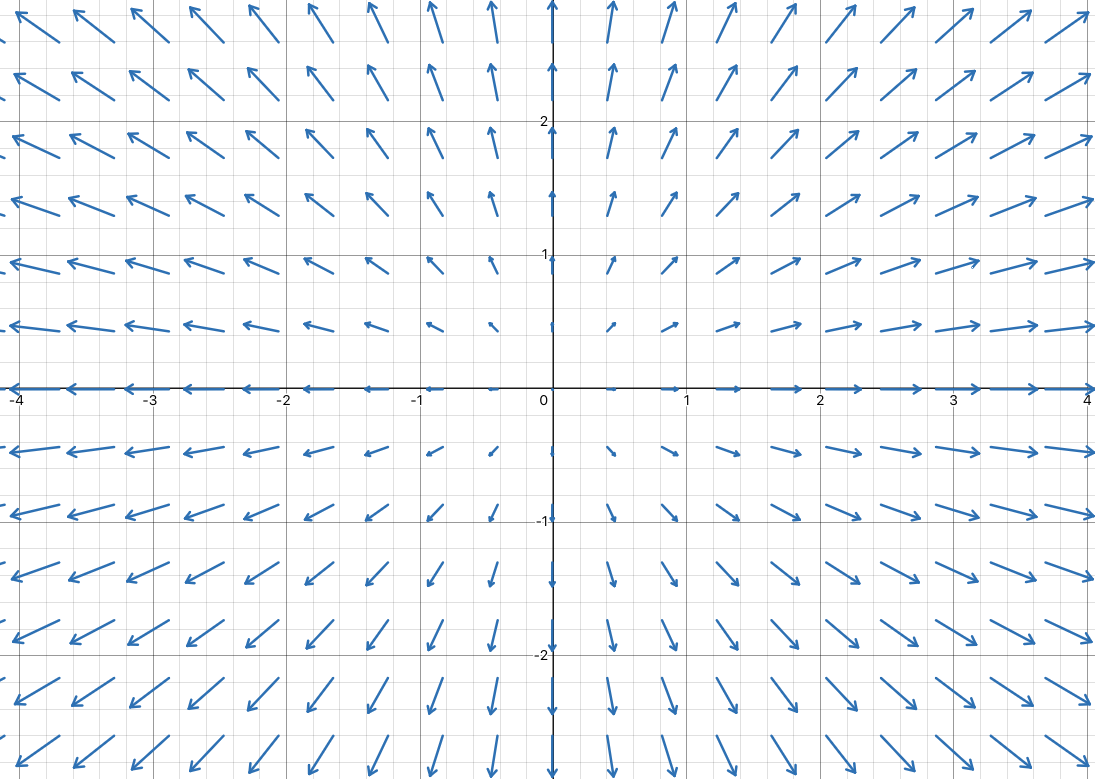
\includegraphics[height=0.4\textwidth]{assets/physics-2/vector-field-example.png}
        \caption{The arrow representation of $\vec v$ when $z = 0$.}
        \label{fig:field_source_0}
    \end{figure}
\end{example}

Some vector fields have \say{special points} where there are an infinite number of field lines going through it:
\begin{itemize}
    \item If all the lines go into that point we call such point \textbf{source} (the point $(0,0,0)$ is a source for \Cref{ex:vec-field});
    \item If all the lines go out of that point we call such point \textbf{sink} (use the field $\vec v(x, y, z) = -x \hat x - y \hat y - z \hat z$ as an example).
\end{itemize}
It is possible for some vector fields to have no sources or sinks. Some patterns that can arise are \textit{loops} or \textit{straight lines}.

\subsection{Operations over fields}

\begin{definition}{Gradient of a scalar field}{gradient-scalar}
    We define the gradient as
    \begin{equation}
        \grad f = \pdv{f}{x} \hat{x} + \pdv{f}{y} \hat{y} + \pdv{f}{z} \hat{z}
    \end{equation}

    We can also define the differential of a field as follows (where $\dd{l} = \dd{x} \hat{x} + \dd{y} \hat{y} + \dd{z} \hat{z} $):
    \begin{equation}
        \dd{f} = \pdv{f}{x} \dd{x} + \pdv{f}{y} \dd{y} + \pdv{f}{z} \dd{z} = \grad f \cdot \dd{\vec l}
    \end{equation}
\end{definition}

The gradient of a field is somewhat the equivalent of the derivative for 1D functions.

\begin{proposition}{Properties of the gradient}{props-gradient}
    \begin{enumerate}[label=\roman*.]
        \item $\grad f$ is orthogonal to the level curves;
        \item $\grad f$ points in the direction of the steepest ascent;
    \end{enumerate}
\end{proposition}

\begin{definition}{Directional derivative}{directional-derivative}
    The directional derivative is the slope of the field in the direction $\vec l$.
    \begin{equation}
        \dv{f}{l} = \grad \cdot \dd{\vec l}
    \end{equation}
\end{definition}

\begin{definition}{Gradient (nabla) operator}{nabla-operator}
    We define the nabla operator as
    \begin{equation}
        \grad = \pdv{}{x} \hat{x} + \pdv{}{y} \hat{y} + \pdv{}{z} \hat{z}
    \end{equation}
\end{definition}

This operator is particularly useful because we can treat it basically like a vector: when we multiply the $\grad$ with a vector field $f$ we get the gradient field of $f$.

\begin{definition}{Divergence}{divergence}
    Let $\vec v$. Then
    \begin{align}
        \div \vec v & = \left( \pdv{}{x} \hat{x} + \pdv{}{y} \hat{y} + \pdv{}{z} \hat{z} \right) \cdot \left( v_x \hat x + v_y \hat y + v_z \hat z\right) \\
                    & = \pdv{v_x}{x} + \pdv{v_y}{y} + \pdv{v_z}{z}
    \end{align}
\end{definition}

The intuition behind divergence is to measure how much a field \say{spreads out} from the point where it is measured.

\begin{example}{}{}
    Take $\vec v$ as in \Cref{fig:field_source_0}. Then
    \begin{equation}
        \div \vec v = \pdv{x}{x} + \pdv{y}{y} + \pdv{z}{z} = 3
    \end{equation}

    We have that the divergence for this field is always positive therefore the arrows always go further away from each other.
\end{example}

\begin{example}{Solenoidal field}{solenoidal-field}
    Let $\vec v = \hat z$. We have $\div \vec v = 0$.

    Fields with zero divergence are called solenoidals.
\end{example}

\begin{definition}{Curl}{curl}
    Let $\vec v$ be a vector field. Then
    \begin{equation}
        \curl \vec f = \det\begin{vmatrix}
            \hat x    & \hat y    & \hat z    \\
            \pdv{}{x} & \pdv{}{y} & \pdv{}{z} \\
            v_x       & v_y       & v_z
        \end{vmatrix}
    \end{equation}
\end{definition}

The intuition behind curl is to measure how much a vector field rotates or spins around the point where we compute it.

\begin{proposition}{Linearity}{linearity-of-grad}
    $\grad(\mathord{\cdot})$, $\div(\mathord{\cdot})$, and $\curl(\mathord{\cdot})$ are linear operators.
\end{proposition}

\begin{proposition}{Leibniz rule}{leibniz-rule}
    \begin{equation}
        \grad{fg} = (\grad f)g + f (\grad g)
    \end{equation}
\end{proposition}

\subsubsection{Higher order derivatives}
\label{sec:higher-order-derivatives}

\begin{enumerate}
    \item \textit{Divergence of gradient}
          (also called \textit{laplacian}):

          \begin{align}
              \div (\grad \vec f) & = \left( \pdv{}{x} \hat{x} + \pdv{}{y} \hat{y} + \pdv{}{z} \hat{z} \right) \cdot \left( \pdv{f}{x} \hat{x} + \pdv{f}{y} \hat{y} + \pdv{f}{z} \hat{z} \right) \\
                                  & = \pdv[2]{f}{x} + \pdv[2]{f}{y} + \pdv[2]{f}{z} = \grad^2(f)
          \end{align}

    \item \textit{Curl of gradient}: $\curl(\grad f) = 0$ (Schwartz theorem holds).
    \item \textit{Gradient of divergence}: $\grad (\div \vec V)$ is usually not useful.
    \item \textit{Divergence of curl}: $\div (\curl \vec v) = 0$
    \item \textit{Curl of curl}: (not so frequent)
          \begin{equation}
              \curl (\curl \vec f) = \grad (\div \vec v) - \grad^2(\vec v)
          \end{equation}
          where $\grad^2(\vec v) = (\grad^2 v_x \hat x + \grad^2 v_y \hat y + \grad^2 v_z \hat z)$ is called the laplacian vector operator.
\end{enumerate}

\subsection{Integrals}

\subsubsection{Line integrals}

\begin{definition}{Line integral}{line-integral}
    Let $f$ be a scalar field and $\vec v$ a vector field.
    \begin{enumerate}
        \item $\int_C f \dd{s}$
        \item $\int_C \vec v \dd{\vec l}$
    \end{enumerate}
    where $\dd{\vec l}$ is tangent to $C$ at every point.
\end{definition}

Note that if $C$ is closed we will write $\oint$ instead of $\int$.

Moreover, some fields $\vec v$ are such that $\int_C \vec v \dd{\vec l}$ does not depend on $C$ but only on its endpoints.
These are called \textbf{conservative fields}.

\subsubsection{Surface integral}

Let a vector field $\vec v$ and an open surface $S$.
We define $\dd{\vec S}$ the infinitesimal area oriented normal to $S$: $\dd{\vec S} = \dd{S} \vec n$.

Then define the \textit{infinitesimal flux} over $S$ as
\begin{equation}
    \dd{\Phi_S(\vec v)} = \vec v \cdot \dd{\vec S}
\end{equation}

\begin{definition}{Flux}{flux}
    The flux of $\vec v$ over $S$ is defined as
    \begin{equation}
        \Phi_S(\vec v) = \int_S \dd{\Phi_S(\vec v)} = \int \vec v \cdot \dd{\vec S}
    \end{equation}
\end{definition}

Again, if $S$ is a closed surface (like a sphere) we use $\oint$ instead of $\int$.
By convention, if $S$ is closed $\vec n$ goes outwards.

Moreover, we will commonly refer to $C$ as the boundary of $S$.

\subsubsection{Volume integral}

\begin{definition}{Volume integral}{volume-integral}
    Let $f$ be a scalar field and $V \in \R^3$.
    We want to define $I = \int_V f \dd{\tau}$ where $\dd{\tau} = \dd{x} \dd{y} \dd{z}$.

    If $\vec g$ is a vector field we define the integral as
    \begin{equation}
        \vec I = \int_V \vec g(x, y, z) \dd{\tau} = \int_V g_x (x, y, z) \dd{x} \hat x + \int_V g_y (x, y, z) \dd{y} \hat y + \int_V g_z (x, y, z) \dd{z} \hat z
    \end{equation}
\end{definition}

\subsection{Theorems for \texorpdfstring{$\grad(\mathord{\cdot})$, $\div(\mathord{\cdot})$, and $\curl(\mathord{\cdot}) $}{gradient, divergence and curl}}

\subsubsection{Gradient}

\begin{theorem}{Fundamental theorem of gradient}{fundamental-gradient}
    Let $f$ be a gradient field and $C$ be a path. We have
    \begin{equation}
        \int_C \dd{f} = \int_A^B \grad f \cdot \dd{\vec l} = f(B)- f(A)
    \end{equation}
\end{theorem}

\begin{corollary}{}{}
    If $\vec v = \grad f$ then $\vec v$ is conservative.
\end{corollary}

\begin{corollary}{}{}
    If $C$ is closed and $\vec v = \grad f$ we have
    \begin{equation}
        \oint \vec v \cdot \dd{\vec l} = \oint \grad f \cdot \dd{l} = 0
    \end{equation}
\end{corollary}

\subsubsection{Divergence}

\begin{theorem}{Divergence theorem}{divergence-theorem}
    Let $V$ be a volume, $S$ be a surface corresponding to that volume and $\vec v$ a vector field.
    Then
    \begin{equation}
        \int_V \left(\div \vec v\right) = \oint_S \vec v \cdot \dd{\vec S}
    \end{equation}
\end{theorem}

\begin{proof}
    We have done a partial proof in the case of a cube in Physics 1.
\end{proof}

\begin{corollary}{}{}
    If $\vec v$ is solenoidal
    \begin{enumerate}
        \item $\oint_S \vec v \cdot \dd{\vec S} = 0 \enspace \forall S$
        \item $\int_S \vec v \cdot \dd{S}$ is independent of $S$ but only on the boundary line of $S$
        \item Let $\vec v = \curl \vec A$ where $\vec A$ is a vector field. Then $\div \vec v = \div (\curl \vec A) = 0$
    \end{enumerate}
\end{corollary}

\begin{proof}
    \skiplineafterproof
    \begin{enumerate}
        \item Trivial from theorem and definition of solenoidal.
        \item
              For any $S_1$ open we can find another $S_2$ open with the same boundary line.
              Let $S = S_1 \cup S_2$, then $S$ is closed.
              By the divergence theorem we can write
              \begin{equation}
                  \oint_S \vec v \cdot \dd{\vec S} = \int_V \left(\div \vec v\right) = 0 = \int_{S_1} \vec v \cdot \dd{\vec S} + \int_{S_2} \vec v \cdot \dd{\vec S}
              \end{equation}
              This means that $\abs{\Phi_{S_1}(\vec v)} = \abs{\Phi_{S_2} (\vec v)}$.
        \item This is a consequence of the theorem and the results of \cref{sec:higher-order-derivatives}.
    \end{enumerate}
\end{proof}

\subsubsection{Curl}

\begin{theorem}{Stokes' theorem}{stokes}
    Let $\vec v$ be a vector field, $S$ an open surface, $C$ the boundary line of $S$.
    Then
    \begin{equation}
        \int_S (\curl \vec v) \cdot \dd{\vec S} = \oint_C \vec v \cdot \dd{\vec l}
    \end{equation}
    and the direction of $C$ depends on the direction of the normals of $S$ by the right-hand rule.
\end{theorem}

The intuition behind the theorem is that if we consider the total \say{rotation} in the surface it will be equal to the total \say{diraction} of the vectors at the boundary.

\begin{proof}
    We will consider a surface that can be decomposed in rectangles.
    Consider a rectangle with vertices $P_1,P_2,P_3,P_4$ on the $yz$ plane. Let $\dd{y}$ be the \say{base} of the rectangle, $\dd{z}$ its height and $A = (x, y, z)$ the center of the rectangle.

    Now we want to compute the line integral over the boundary of the rectangle going counterclockwise:
    \begin{align}
        P_1 P_2: \quad & \dd{\vec l} = \dd{y} \hat y \implies \vec v \cdot \dd{\vec l} = v_y\left(x, y, z - \frac{\dd{z}}{2}\right)\dd{y} \approx \left[v_y(x, y, z) \dd{y} - \pdv{v_y(x, y, z)}{z} \frac{\dd{z}}{2}\right] \dd{y}    \\
        P_3 P_4: \quad & \dd{\vec l} = -\dd{y} \hat y \implies \vec v \cdot \dd{\vec l} = -v_y\left(x, y, z - \frac{\dd{z}}{2}\right)\dd{y} \approx -\left[v_y(x, y, z) \dd{y} - \pdv{v_y(x, y, z)}{z} \frac{\dd{z}}{2}\right] \dd{y} \\
        P_2 P_3: \quad & \dd{\vec l} = \dd{z} \hat z \implies \vec v \cdot \dd{\vec l} = v_z\left(x, y - \frac{\dd{y}}{2}, z\right)\dd{y} \approx \left[v_z(x, y, z) \dd{z} - \pdv{v_z(x, y, z)}{y} \frac{\dd{y}}{2}\right] \dd{z}    \\
        P_4 P_1: \quad & \dd{\vec l} = -\dd{z} \hat z \implies \vec v \cdot \dd{\vec l} = -v_z\left(x, y - \frac{\dd{y}}{2}, z\right)\dd{y} \approx -\left[v_z(x, y, z) \dd{z} - \pdv{v_z(x, y, z)}{y} \frac{\dd{y}}{2}\right] \dd{z}
    \end{align}
    where the $\approx$ are due to a taylor expansion.

    By summing up all the terms we get that many terms cancel out:
    \begin{equation}
        P_1P_2 + P_2P_3 + P_3P_4 + P_4P_1 = \left( \pdv{v_z}{y} - \pdv{v_y}{z} \right) \dd{y} \dd{z} = \left( \curl \vec v \right)_x \dd{y} \dd{z}
    \end{equation}

    \textit{A complete proof would require the same procedure on the $xy$ and $xz$ planes.}
\end{proof}

\begin{corollary}{}{}
    The theorem doesn't say anything about $S$ itself, just the boundary $C$.
    Therefore we can say
    \begin{equation}
        \int_S (\curl \vec v) \cdot \dd{\vec S} \text{ only depends on the boundary line of } S
    \end{equation}

    Moreover
    \begin{equation}
        \oint_S (\curl \vec v) \cdot \dd{\vec S} = 0
    \end{equation}
\end{corollary}

\begin{theorem}{Fundamental theorem for irrotational fields}{irrotational-fields}
    Let $\vec v$ such that $\curl \vec v = 0$ everywhere.
    Then:
    \begin{enumerate}
        \item $\oint_C \vec v \cdot \dd{\vec l} \enspace \forall C \text{ closed}$.
        \item $\int_A^B \vec v \cdot \dd{\vec l}$ is independent of the slope of the path.
        \item There exists $f$ such that $\vec v = \grad f$.
    \end{enumerate}
\end{theorem}

\subsection{Dirac delta function}

\subsubsection{Motivation}

Let $\vec v$ be a vector field defined as
\begin{equation}
    \vec v = \frac{\vec r}{r^3} = \frac{x \hat x + y \hat y + z \hat z}{\left( x^2 + y^2 + z^2\right)^{\frac{3}{2}}} \in \R^3 \setminus (0,0,0)
\end{equation}

We want to compute its divergence.
\begin{equation}
    \pdv{v_x}{x} = \frac{1}{\left( x^2 + y^2 + z^2\right)^{\frac{3}{2}}} - \frac{3}{2}\frac{2 x^2}{\left( x^2 + y^2 + z^2\right)^{\frac{5}{2}}} = \frac{-2x^2 + y^2 + z^2}{\left( x^2 + y^2 + z^2\right)^{\frac{5}{2}}}
\end{equation}

Similarly we get
\begin{align}
    \pdv{v_x}{x} & = \frac{x^2 - 2y^2 + z^2}{\left( x^2 + y^2 + z^2\right)^{\frac{5}{2}}} \\
    \pdv{v_x}{x} & = \frac{x^2 + y^2 - 2z^2}{\left( x^2 + y^2 + z^2\right)^{\frac{5}{2}}}
\end{align}
and by adding up all the partial derivatives we get that $\div \vec v = 0$.

Now let's use the divergence theorem to compute the flux of $\vec v$ over a sphere:
\begin{equation}
    \oint_S \vec v \cdot \dd{\vec S} = \int_V \div \vec v \dd{\tau} {\color{red}= 0}
    \label{eq:dirac-wrong}
\end{equation}

This would look correct but let's also compute this without the divergence theorem.
Using spherical coordinates we write
\begin{equation}
    \dd{\vec S} = \dd{S}\hat r = R^2 \sin\theta \dd{\theta} \dd{\phi} \hat r
\end{equation}
Now we notice that $\dd{S}$ is always at the same distance from the center of the sphere and
\begin{equation}
    \oint_S \vec v \cdot \dd{\vec S} = \int \frac{R}{R^3} \dd{S} = \frac{1}{R^2} \int \dd{S} = \frac{1}{R^2} \cdot 4 \pi R^2
\end{equation}
where $\int \dd{S}$ is the area of the sphere, therefore we get a result of $4\pi$ which conflicts with the result we got from the divergence theorem.

The issue is that we have a singularity at $(0,0,0)$ where the divergence is not $0$.

\subsubsection{1D Dirac delta function}

To simplify we start by the 1D case.
\begin{definition}{1D Dirac delta function}{1d-dirac-delta}
    \begin{equation}
        \delta(x) = \begin{cases}
            0      & x \ne 0          \\
            \infty & \text{if } x = 0
        \end{cases}  \quad, \quad \int_{-\infty}^{\infty} \delta(x) \dd{x} = 1
    \end{equation}
\end{definition}

A way to obtain this function is as the limit of a sequence of functions. Define
\begin{equation}
    R_n(x) = n \cdot 1_{[-\frac{1}{2n}, \frac{1}{2n}]}(x)
\end{equation}
the rectangle of width $\frac{1}{n}$ and height $n$.
Indeed the integral of this function is $1$ and as we take $\lim_{n \to \infty} R_n(x) = \delta(x)$.

Another way to obtain $\delta(x)$ is taking a gaussian distribution with $\mu = 0$ and take $\lim_{\sigma^2 \to 0}$.

\begin{proposition}{Properties of the Dirac delta functions}{prop-1D-dirac-delta}
    We have that $f(x)\delta(x) = f(0) \delta(x)$.
    Moreover, under the integral we get
    \begin{equation}
        \int_{-\infty}^{\infty} f(x) \delta(x - x_0) \dd{x} = \int_{-\infty}^{\infty} f(x_0) \delta(x) \dd{x} = f(x_0)
    \end{equation}
    for a fixed $x_0$.
\end{proposition}

To be able to apply this property we have to make sure that the \say{spike} is within the boundary of integration.

\subsubsection{3D Dirac delta function}

Now we are ready to go back to the 3D version:
\begin{definition}{3D Dirac delta function}{dirac-delta}
    \begin{equation}
        \delta^{(3)}(\vec r) = \delta(\vec r) = \delta(x) \delta(y) \delta(z)
    \end{equation}
    that is, the product of the 1D version of the dirac delta as in \cref{def:1d-dirac-delta}.
\end{definition}

Here we have as well that the integral is $1$:
\begin{equation}
    \int_{\R^3} \delta(\vec r) \dd{x} \dd{y} \dd{z} = \int_{\R^3} \delta(x) \delta(y) \delta(z) \dd{x} \dd{y} \dd{z} = 1 \cdot 1 \cdot 1 = 1
\end{equation}

Now we can solve the mystery of \cref{eq:dirac-wrong}
\begin{equation}
    \label{eq:dirac-delta-ok}
    \div \left( \frac{\hat r}{r^3} \right) = 4 \pi \delta(\vec r)
\end{equation}

\subsection{Change of coordinates}

\subsubsection{Spherical coordiante}

\begin{definition}{Spherical coordinates}{spherical-coordiantes}
    Let $\vec r = x \hat x + y \hat y + z \hat z$.
    We use the following transformation:
    \begin{equation}
        \begin{cases}
            x = r \sin \theta \cos \varphi & r \in [0, \infty)     \\
            y = r \sin \theta \sin \varphi & \theta \in [0, \pi]   \\
            z = r \cos \theta              & \varphi \in [0, 2\pi]
        \end{cases}
    \end{equation}
    where $r$ is the distance of the point with the origin, $\theta$ is the angle that $\vec r$ makes with the $z$ axis, and $\varphi$ is the angle on the $xy$-plane that the projection makes with the $y$ axis.
\end{definition}

To define directions in this coordinate system we fix two coordinates and we slightly increase the other: the \say{movement} we obtain is the direction we want:
\begin{itemize}
    \item $\hat r$ is the radial direction, obtained by slightly increasing $r$
    \item $\hat \theta$ is obtained by increasing $\theta$
    \item $\hat \varphi$ is obtained by increasing $\varphi$
\end{itemize}

\begin{proposition}{Jacobian of spherical change of coordinates}{jacobian-spherical}
    We want to compute $\dd{\vec l}$ given $\dd{x} + \dd{y} + \dd{z}$:
    \begin{itemize}
        \item $\dd{l}_r = \dd{r}$
        \item $\dd{l}_\theta = r \dd{\theta}$
        \item $\dd{l}_\varphi = r \sin \theta \dd{\varphi}$
    \end{itemize}

    Therefore
    \begin{equation}
        \dd{\tau} = \dd{x} \dd{y} \dd{z} = r^2 \sin \theta \dd{r} \dd{\theta} \dd{\varphi}
    \end{equation}
\end{proposition}

\subsubsection{Cylindircal coordinates}

\begin{definition}{Cylindircal coordinates}
    Let $\vec r = x \hat x + y \hat y + z \hat z$.
    We use the following transformation:
    \begin{equation}
        \begin{cases}
            x = s \cos \varphi & s \in [0, \infty)       \\
            y = s \sin \varphi & \varphi \in [0, \pi]    \\
            z = z              & z \in (-\infty, \infty)
        \end{cases}
    \end{equation}
\end{definition}

\begin{proposition}{Jacobian of cylindircal change of coordinates}{jacobian-cylindircal}
    \begin{equation}
        \dd{\tau} = \dd{x} \dd{y} \dd{z} = s \dd{s} \dd{\varphi} \dd{z}
    \end{equation}
\end{proposition}

\section{Electrostatics}

\subsection{Introduction}

Franklin was the first one to show that rubbing a piece of glass with fur you get a positive charge, while if you do it with amber you get a negative charge.
Fur would always get the opposite charge (\emph{conservation of charge}).
He noticed that same charge repel while different charges attract.

Charge is measured in Coulomb ($\si{\coulomb}$).
To measure charge we use the \emph{electroscope}:
this instrument will get charged by contact and since alike charges repel we can measure the angle the gold foil create to measure the charge.

\begin{figure}[H]
    \centering
    \includesvg[height=0.4\textwidth]{assets/physics-2/electroscope.svg}
    \caption{Drawing of an electroscope}
\end{figure}

The \textbf{general problem of electrostatics} is to compute the force due to some \emph{source charges} $q_1, \dots, q_n$ on a \emph{test charge} $Q$.

\begin{proposition}{Charge is quantized}{quantization-charge}
    The smallest charge possible is the charge of an electron:
    \begin{equation}
        Q_e = 1.6 \cdot 10^{-19} \si{\coulomb}
    \end{equation}
\end{proposition}

\begin{proposition}{Superposition principle}{superposition-principle}
    If we have $n$ charges, the total force applied by those particles is
    \begin{equation}
        \vec F = \vec F_1 + \dots + \vec F_n
    \end{equation}
\end{proposition}

But even in the case of $n = 1$ it is not easy to compute $\vec F$ because it not only depends on $\vec r$ but also $\vec v_q$ and $\vec a_q$.
This is why we invented electrostatics, where charges do not move.

\subsection{Coulomb's law}

\begin{theorem}{Coulomb's law}{coulomb-law}
    Let the distance between the two charges be $ \vec{\Delta r} = \vec {r'} - \vec r$.
    Then the force applied on the two charges is
    \begin{equation}
        \vec F = k \frac{qQ}{\Delta r^2} \hat{\Delta r}
    \end{equation}
    where $k$ is a constant:
    \begin{equation}
        k = \frac{1}{4\pi \varepsilon_0} \simeq 9 \cdot 10^9 \si{\newton \meter \squared \per \coulomb \squared}
    \end{equation}
    and $\varepsilon_0$ is another constant called \textbf{permittivity in vacuum}.
\end{theorem}

Note that, compared to gravity, electric force is in the order of $10^{39}$ times stronger.

\begin{definition}{Electric field (of a point charge)}{electric-field-point}
    \begin{equation}
        \vec E(\vec r) = \frac{\vec F}{Q} = k \frac{q}{\Delta r^2} \hat{\Delta r}
    \end{equation}

    This is particularly useful because it is independent of the test charge.
\end{definition}

If the charge is positive the field will have positive divergence, if negative it will have negative divergence.
Moreover, note that the electric field gets its field lines from $\frac{r^2}{\hat r}$ as in \Cref{eq:dirac-delta-ok}.

\begin{definition}{Electric field (continuous charge distribution)}{electric-field-cont}
    Consider a small $\dd{\tau}$ where we can consider to have a constant point charge of $\dd{q}$.
    Then
    \begin{align}
        \dd{\vec E} & = \frac{1}{4\pi \varepsilon_0} \frac{\dd{q}}{\Delta r^2} \hat{\Delta r}                             \\
        \vec E      & = \int_R \dd{\vec E} = \frac{1}{4\pi \varepsilon_0} \int_R \frac{\dd{q}}{\Delta r^2} \hat{\Delta r}
    \end{align}
    where $R$ is the region where the charge is.
\end{definition}

We now have three cases.
\begin{enumerate}
    \item \emph{$R$ is one-dimensional}.
          Let $\lambda$ be the 1D density of charge:
          \begin{equation}
              \lambda(\vec {r'}) = \dv{q}{l} \implies \dd{q} = \lambda (\vec {r'}) \dd{l}
          \end{equation}
    \item \emph{$R$ is a surface of charge}.
          \begin{equation}
              \sigma(\vec {r'}) = \dv{q}{S}
          \end{equation}
    \item \emph{$R$ is a volume density of charge}.
          \begin{equation}
              \rho(\vec {r'}) = \dv{q}{\tau}
          \end{equation}
\end{enumerate}
Similarly to the first case, in the other two we define the density of charge in the respective dimension and substitute $\dd{q}$ in the field equation.

\begin{example}{Staight line of constant charge}{straight-line-const-charge}
    Consider a straight line of length $2L$ and of constant charge $\lambda(\vec r) = \lambda$.
    Compute the electric field at $P(0,z)$.

    \begin{figure}[H]
        \centering
        \includesvg[height=0.4\textwidth]{assets/physics-2/ex-electric-field-straight-line.svg}
        \caption{Illustration of the problem}
    \end{figure}
\end{example}

\begin{proof}[Solution]
    First, consider the infinitesimal change in the electric field $\dd{\vec E}$ due to a small $\dd{l}$ difference length of the line.
    As we know, a length of $\dd{l}$ carries a charge of $\dd{q} = \lambda \dd{l}$, hence adding $\dd{l}$ on each side of the line will result in $\dd{\vec E_1}$ and $\dd{\vec E_2}$.
    We can compute the total $\dd{\vec E}$ as
    \begin{align}
        \dd{\vec E} & = \dd{\vec E_1} + \dd{\vec E_2}                                                \\
                    & = 2 \dd{E_1} \cos \theta \hat z                                                \\
                    & = 2\oneover{4 \pi \varepsilon_0} \frac{\dd{q}}{r^2} \cos \theta \hat z         \\
                    & = 2\oneover{4 \pi \varepsilon_0} \frac{\lambda \dd{l}}{r^2} \cos \theta \hat z
    \end{align}

    Next we want to write everything in terms of $\theta$ such that we can integrate over it.
    We have
    \begin{gather}
        r         = \frac{z}{\cos \theta}                                      \\
        l(\theta) = z \tan \theta                                              \\
        \dd{l}    = \dd{z \tan \theta} = \frac{z}{\cos^2 \theta} \dd{\theta}
    \end{gather}
    and rewrite $\dd{E}$ accordingly
    \begin{align}
        \dd{E} & = 2\oneover{4 \pi \varepsilon_0} \frac{\lambda \frac{z}{\cos^2 \theta} \dd{\theta}}{\frac{z^2}{\cos^2 \theta}} \cos \theta \hat z \\
               & = \oneover{2 \pi \varepsilon_0} \frac{\lambda}{z} \dd{\theta} \cos \theta \hat z
    \end{align}

    Now we can integrate in order to find the field
    \begin{align}
        \vec E & = \int \dd{\vec E}                                                                                                       \\
               & = \oneover{2 \pi \varepsilon_0} \frac{\lambda}{z} \hat z \underbrace{\int_0^{\frac{\pi}{2}} \dd{\theta} \cos \theta}_{1} \\
               & = \oneover{2 \pi \varepsilon_0} \frac{\lambda}{z} \hat z
    \end{align}
\end{proof}

\begin{example}{uniformly charged ring}{uniformly-charged-ring}
    Consider a ring of radius $R$ and of constant charge $\lambda(\vec r) = \lambda$.
    Compute the electric field at $P(0,z)$.

    \begin{figure}[H]
        \centering
        \includesvg[height=0.4\textwidth]{assets/physics-2/ex-electric-field-ring.svg}
        \caption{Illustration of the problem}
    \end{figure}
\end{example}

\begin{proof}[Solution]
    We proceed similarly to \Cref{ex:straight-line-const-charge}: first we need to compute $\dd{\vec E}$.
    \begin{align}
        \dd{\vec E} & = \dd{\vec E_1} + \dd{\vec E_2} = 2 \dd{E_1} \cos \theta \hat z               \\
                    & = \frac{2}{4 \pi \varepsilon_0} \frac{\lambda \dd{l}}{r^2} \cos \theta \hat z
    \end{align}

    This time we notice that $\theta$ does not depend on $\dd{l}$, therefore we can compute the integral quite easily as follows:
    \begin{align}
        \vec E & = \int \dd{\vec E} = \frac{2}{4 \pi \varepsilon_0} \frac{\lambda}{r^2} \underbrace{\cos \theta}_{z/r} \hat z \underbrace{\int \dd{l}}_{\pi R} \\
               & = \frac{1}{4 \pi \varepsilon_0} \frac{\lambda (2\pi R) z}{\left(\sqrt{R^2 + z^2}\right)^3} \hat z
    \end{align}
\end{proof}

\begin{example}{uniformly charged disk}{uniformly-charged-disk}
    Consider a disk of radius $R$ and of constant charge $\sigma(r') = \sigma$.
    Compute the electric field at $P(0,z)$.

    \begin{figure}[H]
        \centering
        \includesvg[height=0.4\textwidth]{assets/physics-2/ex-electric-field-disk.svg}
        \caption{Illustration of the problem}
    \end{figure}
\end{example}

\begin{proof}[Solution]
    The trick is to divide the disk into rings of radius $r \in [0, R]$ with thickness $\dd{r}$, therefore the charge of each ring is
    \begin{equation}
        \dd{q}_\text{ring} = \sigma (2 \pi r) \dd{r}
    \end{equation}
    and we can take the result of \Cref{ex:uniformly-charged-ring} and substitute
    \begin{equation}
        \dd{\vec E}_\text{ring} = \frac{1}{4 \pi \varepsilon_0} \frac{\sigma (2 \pi r) z}{\left(\sqrt{r^2 + z^2}\right)^3} \dd{r} \hat z
    \end{equation}

    Finally, we can integrate in order to get the final result
    \begin{align}
        \vec E & = \int \dd{\vec E}_\text{ring}                                                                                    \\
               & = \frac{1}{4 \pi \varepsilon_0} \sigma(2 \pi) z  \hat z \int_0^R \frac{r}{\left(\sqrt{r^2 + z^2}\right)^3} \dd{r} \\
               & = \frac{\sigma z}{2 \varepsilon_0} \hat z \int_0^R \frac{r}{\left(r^2 + z^2\right)^{\frac{3}{2}}} \dd{r}          \\
               & = \frac{\sigma z}{2 \varepsilon_0} \hat z \left[ -\oneover{\sqrt{z^2 + r^2}} \right]_0^R                          \\
               & = \frac{\sigma z}{2 \varepsilon_0} \left[ \oneover{z} - \oneover{\sqrt{z^2 + R^2}} \right] \hat z
    \end{align}

    Notably, the case where $R \to \infty$ is interesting, meaning the disk becomes a plane.
    In this situation we have that the above equation becomes
    \begin{equation}
        \vec E = \frac{\sigma}{2 \varepsilon_0} \hat z
    \end{equation}
\end{proof}


\subsection{Gauss's law}

\begin{theorem}{Gauss's law}{gauss-law}
    Let $S$ be a closed surface and $Q_\text{enclosed}$ be the total charge enclosed in $S$.
    The flux of the electric flux going through $S$ is
    \begin{equation}
        \Phi_S(\vec E) = \oint_S \vec E \cdot \dd{\vec S} = \frac{Q_\text{enclosed}}{\varepsilon_0}
    \end{equation}
\end{theorem}

We will start with an easy example.
We can consider the field generated by a point charge $q$ at the origin and a sphere $S$ centered at the origin with radius $R$.
We have
\begin{align}
    \vec E      & = \oneover{4 \pi \epsilon_0} \frac{q}{r^2} \hat r \\
    \dd{\vec S} & = \dd{S} \hat r
\end{align}
which are in the same direction, so the dot product is just the product of the moduli.
\begin{align}
    \Phi_S(\vec E) & = \oint_S \vec E \cdot \dd{\vec S}                                                                                         \\
                   & = \oint_S E(r = R) \dd{S}                                                                                                  \\
                   & = \oneover{4 \pi \epsilon_0} \frac{q}{R^2} \underbrace{\oint_\text{sphere} \dd{S}}_{\text{surface of sphere } = 4 \pi R^2} \\
                   & = \frac{q}{\varepsilon_0}
\end{align}

From this easy case we will add the following extensions (without proof):
\begin{enumerate}[label=\roman*.]
    \item $q$ is not in the origin, with $q \subset S$, $\implies \Phi_S(\vec E)=\frac{q}{\varepsilon_0}$
    \item $S$ is not a sphere, with $q \subset S$, $\implies \Phi_S(\vec E)=\frac{q}{\varepsilon_0}$
    \item $q \not \subset S \implies \Phi_S(\vec E)= 0$
    \item These results remain valid even with a discrete number or a continuously distribution of charge
\end{enumerate}

This law is useful in particular if we have some symmetries.
In this course we will cover the following symmetries:
\begin{enumerate}
    \item Plane
    \item Spherical
    \item Cylindrical
\end{enumerate}

\begin{example}{Electric field of a sphere}{electric-field-sphere-symmetry}
    Consider a sphere with charge $q$, uniformly distributed ($\rho(\vec{r'}) = \rho$).
    Find $\vec E$ outside the sphere ($r \geq R$).
\end{example}

\begin{proof}[Solution]
    Using symmetry, we will determine the direction and where the modulus of $\vec E$ is constant.
    We find out that the direction is $\hat r$ and the modulus is constant at the same distance from the origin, therefore a sphere is the perfect surface to compute the vector field.

    Let $S$ be the surface of the sphere with $r \geq R$. We will first compute the flux and use the result and Gauss's law to compute the field.

    \begin{equation}
        \oint_S \vec E \cdot \dd{\vec S} = \oint_S E\dd{S} = E \oint_S \dd{S} = E 4 \pi r^2
    \end{equation}
    by Gauss law we know that this is equal to $\frac{q}{\varepsilon_0}$:
    \begin{equation}
        E 4 \pi r^2 = \frac{q}{\varepsilon_0} \implies \vec E(\vec r) = \oneover{4 \pi \varepsilon_0} \frac{q}{r^2} \hat r
    \end{equation}

    Note that this is the same field as a point charge $q$.
\end{proof}

\begin{example}{Electric field of a line}{electric-field-cylindircal-symmetry}
    Consider a line with charge $q$, uniformly distributed ($\lambda(\vec{r'}) = \lambda$).
    Find $\vec E$.
\end{example}

\begin{proof}[Solution]
    We can argue by symmetry that the direction of the electric field is pointing away from the line, while the modulus is constant at every point equally distant from the line.

    We choose $S$ to be a cylinder centered around the line, of radius $r$ and of height $L$.

    \begin{equation}
        \Phi_S(\vec E) = \oint_S \vec E \cdot \dd{\vec S} = \cancel{\int_{S_\text{top}} \vec E \cdot  \dd{\vec S}} + \cancel{\int_{S_\text{bottom}} \vec E \cdot  \dd{\vec S}} + \int_{S_\text{lateral}} \vec E \cdot  \dd{\vec S}
    \end{equation}
    where we cancelled the top and bottom surface because $\vec E \perp \dd{\vec S}$.

    Now we can easily compute the flux and apply Gauss law.
    \begin{gather}
        \Phi_S(\vec E) =  E \int_{S_\text{lateral}} \vec \dd{S} = E 2 \pi r L = \frac{\lambda L}{\varepsilon_0}\\
        \implies \vec E(r) = \oneover{2 \pi r} \frac{\lambda}{r} \hat r
    \end{gather}
\end{proof}

\begin{example}{Electric field of a plane}{electric-field-plane-symmetry}
    Consider a plane with uniformly distributed charge ($\sigma(\vec {r'}) = \sigma$).
    Find $\vec E$.
\end{example}

\begin{proof}{Solution}
    First, by symmetry, we notice that the electric field must be perpendicular to the plane, pointing away from it, and it must be constant at the same distance from the plane.

    We choose a cube $S$ of side $L$ in between the plane.
    Notice that on the side surfaces the flux is zero, as $\vec E \perp \dd{\vec S}$.
    Therefore the flux is
    \begin{gather}
        \oint_S \vec E \cdot \dd{\vec S} = 2 A E = \frac{\sigma A}{\varepsilon_0}\\
        \implies E = \frac{\sigma}{2 \varepsilon_0}
    \end{gather}

\end{proof}

\subsubsection{Divergence of \texorpdfstring{$\vec E$}{the electric field}}

\begin{equation}
    \vec E(\vec r) = \oneover{4 \pi \varepsilon_0} \int \frac{\hat{\Delta r}}{\Delta r^2} \rho(\vec{r'}) \dd{\tau'}
\end{equation}

\begin{align}
    \div \vec E(\vec r) & = \oneover{4 \pi \varepsilon_0} \int \div \left(\frac{\hat{\Delta r}}{\Delta r^2} \right) \rho(\vec r) \dd{\tau'} \\
                        & = \oneover{\varepsilon_0} \int \dd{\tau'} \rho(\vec{r'}) \delta(\vec r - \vec{r'})                                \\
                        & = \frac{\rho(\vec r)}{\varepsilon_0}
\end{align}

Note that the fact that $\vec {r'}$ becomes $\vec r$ in the solution is not a typo. This is due to shifting the dirac delta function.

We call this equation \emph{first Maxwell equation} or Gauss law in local form.

\begin{proposition}{Equivalence between first maxwell law and gauss law}{equivalence-maxwell-gauss}
    The following are equivalent:
    \begin{itemize}
        \item $\div \vec E = \frac{\rho}{\varepsilon_0}$
        \item $\oint_S \vec E \cdot \dd{\vec S} = \frac{Q_\text{enclosed}}{\varepsilon_0}$
    \end{itemize}
\end{proposition}

\begin{proof}
    First integrate both sides of Maxwell's first equation, then apply divergence theorem:
    \begin{align}
        \int_V \div \vec E \dd{\tau}     & = \int_V \frac{\rho}{\varepsilon_0}       \\
        \oint_S \vec E \cdot \dd{\vec S} & = \frac{Q_\text{enclosed}}{\varepsilon_0}
    \end{align}
\end{proof}

\subsubsection{Curl of \texorpdfstring{$\vec E$}{the electric field}}
\label{sec:curl-electric}

First we can compute the work of the electric field.
To do so, we want to move to spherical coordinates as it is easier to compute this way it's easier.

\begin{equation}
    \label{eq:potential-electric-point}
    \int_A^B \vec E \cdot \dd{l} = \int_A^B E \cos \theta \dd{l} = \int_A^B E \dd{r} = \frac{q}{4 \pi \varepsilon_0} \int_A^B \frac{1}{r^2} \dd{r} = \frac{q}{4 \pi \varepsilon_0} \left(\oneover{r_A} - \oneover{r_B}\right)
\end{equation}

We notice that if the path is closed the work is $0$, meaning that $\vec E$ is conservative.

By Stokes theorem \cref{thm:stokes} we get that
\begin{equation}
    \curl \vec E = 0
\end{equation}

\subsubsection{Considerations on divergence and curl}

Let some unknown vector field $\vec F$. Define $D$ and $\vec C$ as
\begin{equation}
    \begin{cases}
        D = \div \vec F \\
        \vec C = \curl \vec F
    \end{cases}
\end{equation}
Can we recover $\vec F$ just from $D$ and $\vec C$?

\begin{theorem}{Helmholtz theorem}{helmholtz}
    Let $D = \div \vec F$ and $\vec C = \curl \vec F$ for some vector field $\vec F$.
    Then, if $D, \vec C$ decay to $\infty$ \say{fast enough}
    \begin{equation}
        \vec F = \grad U + \curl \vec W
    \end{equation}
    where
    \begin{align}
        U(\vec r)       & = \oneover{4 \pi} \int \frac{D(\vec(r'))}{\Delta r} \dd{\tau'} \label{eq:helmholtz_1}      \\
        \vec W (\vec r) & = \oneover{4 \pi} \int\frac{\vec C(\vec {r'})}{\Delta r} \dd{\tau'} \label{eq:helmholtz_2}
    \end{align}
\end{theorem}

\subsection{Electric potential and energy}

We know from \cref{sec:curl-electric} that $\vec E$ is conservative:
\begin{equation}
    \vec E = - \grad V \implies \int_C \vec E \cdot \dd{\vec l} = V(A) - V(B)
\end{equation}

The measurement unit of $V$ is $\si{\joule \per \coulomb} = \si{\volt}$ (Volt).
We note the following facts:
\begin{enumerate}[label=\roman*.]
    \item To compute $\vec E$ we only need a scalar function.
    \item We can add any constant $c$ to the potential without altering the field, this means we can choose the point of zero potential.
    \item $V$ satisfies the superposition principle (\cref{prop:superposition-principle})
\end{enumerate}

We will assume
\begin{equation}
    V(\infty) = 0
\end{equation}
this is usually ok, even though we will see some cases where it causes issues.

\begin{example}{Potential of a point charge}{electric-potential-point}
    Compute the potential of a point charge.
\end{example}
\begin{proof}[Solution]
    We have already computed the potential of a point charge in \Cref{eq:potential-electric-point}.

    \begin{equation}
        V(\vec r) = - \int_{\infty}^{\vec r} \vec E \cdot \dd{l} = \oneover{4 \pi \varepsilon_0} \frac{q}{\Delta r}
    \end{equation}
\end{proof}

\begin{example}{Potential of spherical shell}{electric-potential-shell}
    Consider an uniformly charged spherical shell of radius $R$.
    Compute the electric field inside and outside the shell.
\end{example}

\begin{proof}[Solution]
    Outside the shell we can use the flux and symmetry arguments (see \Cref{ex:electric-field-sphere-symmetry}) to get that
    \begin{equation}
        \vec E = \oneover{4 \pi \varepsilon_0} \frac{q}{r^2} \hat r
    \end{equation}
    while inside the shell we have no enclosed charge so the electric field is $0$.

    Now we can compute the potential.
    If we are outside the shell we get
    \begin{equation}
        V(\vec r) = - \int_\infty^{\vec r} \vec E \cdot \dd{\vec l} = - \int_\infty^r \oneover{4 \pi \varepsilon_0} \frac{q}{r^2} \underbrace{\dd{r}}_{\hat r \cdot \dd{\vec l}} = \oneover{4 \pi \varepsilon_0} \frac{q}{r}
    \end{equation}
    while in the inside we have to split the integral between the inside and the outside:
    \begin{equation}
        V(\vec r) = - \int_\infty^{\vec r} \vec E \cdot \dd{\vec l} = -\int_\infty^R \vec E \cdot \dd{\vec l} - \cancelto{0}{\int_R^r \vec E \cdot \dd{\vec l}} = \oneover{4 \pi \varepsilon_0} \frac{q}{R}
    \end{equation}
\end{proof}

TODO: write an example with a full sphere.

\begin{example}{Potential of a plane}{electric-potential-plane}
    Consider a plane with constant charge. Compute its potential.
\end{example}

\begin{proof}[Solution]
    We know from \cref{ex:electric-field-plane-symmetry} that the electric field is
    \begin{equation}
        \vec E = \frac{\sigma}{2 \varepsilon_0} \hat z
    \end{equation}
    We can check that the field has a jump at $z = 0$.

    For a point $P$ we have
    \begin{equation}
        V(P) = - \int_\infty^P \vec E \cdot \dd{\vec l} = - \int^P_\infty \frac{\sigma}{2 \varepsilon_0} \dd{z} = \infty
    \end{equation}
    but this is clearly wrong, as it would mean that the potential is infinity for every point.
    This error is caused by our choice of the zero potential point: choosing $\infty$ only works if the charge is \say{finite}, our plane here is indeed infinite, therefore causing problems.

    To solve thi issue we compute the potential between two points:
    \begin{equation}
        V(B) - V(A) = -\int_A^B \vec E \cdot \dd{\vec l} = -\frac{\sigma}{2 \varepsilon_0}(z_B - z_A)
    \end{equation}
    We see that a safe zero potential point is $z = 0$, by choosing it we get
    \begin{equation}
        V(z) = -\frac{\sigma z}{2 \varepsilon_0}
    \end{equation}
\end{proof}

\subsubsection{Potential of a continuous charge distribution}

We want a way to compute the potential without having to go through the computation of the electric field, we want something similar to Coulomb's law but for potential.

For a discrete charge distribution this is quite easy:
\begin{equation}
    V(\vec r) = \oneover{4 \pi \varepsilon_0} \sum_{k = 1}^n \frac{q_k}{\Delta r_k}
\end{equation}

In the case of a continuously distributed charge we have
\begin{equation}
    \dd{V}(\vec r) = \oneover{4 \pi \varepsilon_0} \frac{\dd{q}}{\Delta r}
\end{equation}
and integrating we get
\begin{equation}
    V(\vec r) = \int \dd{V}(\vec r) = \oneover{4 \pi \varepsilon_0} \int \frac{\dd{q}}{\Delta r} = \oneover{4 \pi \varepsilon_0} \int \frac{\rho(\vec {r'})}{\Delta r} \dd{\tau '}
\end{equation}
which is the result we expected from \Cref{thm:helmholtz} in \Cref{eq:helmholtz_1}.

\subsubsection{Poisson and Laplace equations}

We know that
\begin{equation}
    \begin{cases}
        \div \vec E = \frac{\rho}{\varepsilon_0} \\
        \curl \vec E = 0
    \end{cases}
\end{equation}

Now substituting $\vec E = - \grad V$ in the first equation we get
\begin{equation}
    \label{eq:poisson}
    \div \vec E = - \div (\grad V) = - \laplacian V = \frac{\rho}{\varepsilon_0}
\end{equation}
where $\laplacian{}$ is as defined in \Cref{sec:higher-order-derivatives}.
This is called \textbf{Poisson equation}.

\textbf{Laplace equation} just tells us that if $\rho = 0$ (there is no charge in the region) then
\begin{equation}
    \laplacian V = 0
\end{equation}

\subsubsection{Boundary conditions of \texorpdfstring{$\vec E, V$}{the electric field and the potential}}

Consider a cylinder of base area $\dd A \ll 1$ and height $ \varepsilon \ll 1$ inside a general surface $S$ of constant charge distribution $\sigma$.
We don't assume $S$ is flat.

\begin{align}
    \oint_S \vec E \cdot \dd{\vec S} & = \frac{Q_\text{enc}}{\varepsilon_0} = \frac{\sigma \dd{A}}{\varepsilon_0}                                                                                                                          \\
                                     & = \underbrace{\cancelto{{}_0}{\int_{S_\text{lat}} \vec E \cdot \dd{\vec S}}}_{\propto \varepsilon} + \int_{S_\text{top}} \vec E \cdot \dd{\vec S} + \int_{S_\text{bottom}} \vec E \cdot \dd{\vec S} \\
                                     & = E_\text{top}^\perp \dd{A} - E_\text{bottom}^\perp \dd{A}
\end{align}
that is,
\begin{gather}
    \frac{\sigma \cancel{\dd{A}}}{\varepsilon_0} = E_\text{top}^\perp \cancel{\dd{A}} - E_\text{bottom}^\perp \cancel{\dd{A}}\\
    \implies \frac{\sigma}{\varepsilon_0} = E_\text{top}^\perp - E_\text{bottom}^\perp
\end{gather}

This equation tells us that when we cross a surface we always get a discontinuity in the field.

Now we want to check the tangential component.
Consider a closed path $C$ that crosses the surfaces perpendicularly to it for a distance $\varepsilon \ll 1$, moves a distance $\dd{l}$ tangentially to $S$ and goes back.

\begin{align}
    \oint_C \vec E \cdot \dd{\vec l} & = 0                                                                                \\
                                     & = E_\text{top}^\parallel \dd{l} - E_\text{bottom}^\parallel \dd{l}                 \\
    \implies                         & E_\text{top}^\parallel \cancel{\dd{l}} = E_\text{bottom}^\parallel \cancel{\dd{l}}
\end{align}

In general we can write these two results together as follows:
\begin{equation}
    \label{eq:electric-boundary-condition}
    \vec E_\text{above} - \vec E_\text{below} = \frac{\sigma}{\varepsilon_0} \hat n
\end{equation}

Meanwhile, for the potential we see a different behavior. $V$ is continuous as we cross surfaces' boundaries.

Consider a path $C$ from $A$ to $B$ that crosses a surface in a space $\varepsilon \ll 1$. Let's compute the difference in potential between $A$ and $B$:
\begin{gather}
    V_B - V_A = - \int_A^B \vec E \cdot \dd{\vec l} \propto \varepsilon \to 0 \\
    \implies V_B = V_A
\end{gather}
therefore the potential is continuous.

\subsubsection{Electric dipole}

\begin{figure}[H]
    \centering
    \includesvg[height=0.4\textwidth]{assets/physics-2/electric-dipole.svg}
    \caption{Electric dipole}
    \label{fig:electric-dipole}
\end{figure}

Let us compute the potential in $P$.

\begin{align}
    V(r) & = \frac{q}{4 \pi \varepsilon_0} \left( \oneover{r_+} - \oneover{r_-} \right)                 \\
    r_+  & = \sqrt{r^2 + \left( \frac{d}{2} \right)^2 - \cancel {2} r \frac{d}{\cancel{2}} \cos \theta} \\
    r_-  & = \sqrt{r^2 + \left( \frac{d}{2} \right)^2 + \cancel {2} r \frac{d}{\cancel{2}} \cos \theta} \\
\end{align}

Now we want to see what happens when $P$ is very far away, which means $r \gg d$.
We proceed by taylor expanding:

\begin{align}
    r_+ & = r \sqrt{1 + \left( \frac{d}{2r} \right)^2 - \frac{d}{r} \cos \theta} \approx r \left( 1- \frac{d}{2r} \cos \theta \right)  \\
    r_- & = r \sqrt{1 - \left( \frac{d}{2r} \right)^2 - \frac{d}{r} \cos \theta} \approx r \left( 1 + \frac{d}{2r} \cos \theta \right)
\end{align}
and substituting into $V$ we get
\begin{align}
    V(r) & = \frac{q}{4 \pi \varepsilon_0} \left[ \oneover{r \left( 1- \frac{d}{2r} \cos \theta \right)} - \oneover{r \left( 1 + \frac{d}{2r} \cos \theta \right)} \right] \\
         & \approx  \frac{q}{4 \pi \varepsilon_0 r} \left[ 1 + \frac{d}{2r}\cos\theta - \left( 1- \frac{d}{2r} \cos \theta \right) \right]                                 \\
         & = \frac{1}{4 \pi \varepsilon_0} \frac{q d \cos \theta}{r^2}                                                                                                     \\
         & = \frac{1}{4 \pi \varepsilon_0} \frac{\vec p \cdot \hat r}{r^2}
\end{align}
where we call $\vec p = q d \hat z$ \textbf{dipole moment}.

Now, if we look at what the electric field would do if we follow $\vec E = - \grad V$, we get good results only very far away, otherwise close to the charges the results are wrong.

This result works even in 3D and for any charged volume when $P$ is very far away:
\begin{equation}
    V(r) = \frac{1}{4 \pi \varepsilon_0} \frac{Q_\text{tot}}{r} + \frac{1}{4 \pi \varepsilon_0} \frac{\vec p \cdot \hat r}{r^2} + o\left( \frac{1}{r^3} \right)
\end{equation}

\subsubsection{Energy conservation}

Let $q$ and a test charge $Q$, we want to move $Q$ from $A$ to $B$.

\begin{equation}
    W_E = \int_A^B \vec F_E \cdot \dd{\vec l} = Q \int_A^B \vec E \dd{\vec l} = - Q(V(B)- V(A)) = -\Delta U = - (U(B) - U(A))
\end{equation}
where $U$ is the \emph{potential energy function}.
In this course we will assume energy conservation:
\begin{equation}
    K_A + U_A = K_B + U_B
\end{equation}

\begin{example}{}{}
    Consider an electro accelerated from rest through a potential difference $\Delta V = 100 \si{\volt}$.
    Compute the final speed of $e^-$.
\end{example}

\begin{proof}[Solution]
    We use energy conservation:
    \begin{align}
        E_m^i & = e V_i                     \\
        E^f_m & = \frac{1}{2}mv_f^2 + e V_f
    \end{align}
    which means
    \begin{equation}
        v_f = \sqrt{\frac{2q \Delta V}{m}}
    \end{equation}
\end{proof}

\begin{example}{}{}
    Consider a sphere of radius $R$, total charge $C$ and of charge density $\rho = Ar$ with $r \geq R$ and where $A$ is a parameter.
    \begin{enumerate}
        \item Compute $A$
        \item Compute $\vec E$ inside the sphere
        \item Compute the potential difference between the surface and the origin
    \end{enumerate}
\end{example}

\begin{proof}[Solution]
    We know that we can compute the total charge as
    \begin{gather}
        Q = \int_\text{sphere} \rho \dd{\tau} = A \int r r^2 \sin \theta \dd{\theta} \dd{\varphi} \dd{r} = 4 \pi A \int_0^R r^3 \dd{r} = \pi A R^4 \\
        \implies A = \frac{Q}{\pi R^4}
    \end{gather}

    For the second question we can use gauss law. We choose as a surface a sphere with $r < R$.
    \begin{gather}
        \Phi_S (\vec E) = 4 \pi r^2 E = \frac{q_\text{enc}}{\varepsilon_0} = \frac{1}{\varepsilon_0} \int_0^r \dd{r'} \int_0^\pi \dd{\theta} \int_0^{2 \pi} (\rho)(r')^2 \sin \theta \dd{\varphi}  = \frac{\pi A r^4}{\varepsilon_0} \\
        \implies E = \frac{A}{4 \varepsilon_0} r^2
    \end{gather}

    And for the last question we can just compute the path integral, a straight path will be fine.
    \begin{equation}
        V(R) - V(O) = - \int^R_0 \vec E \cdot \dd{\vec l} = - \frac{A}{4 \varepsilon_0} \int^R_0 r^2 \dd{r} = - \frac{AR^3}{12 \varepsilon_0}
    \end{equation}

    If we don't have any symmetry and we are not able to compute the electric field we can still compute the potential by using the definition.
    The most convenient way to apply it is to choose a point along an axis, compute $\Delta r$ and proceed with the integral in spherical coordinates but this is a much harder procedure.
\end{proof}

\subsection{Work and energy of the electrostatic field}

\subsubsection{2 particles}

If we consider two particles with positive charge at a distance $r$ they will start to move apart.
We conclude that to keep the particles in such position I have to apply a force.
We now want to compute the work needed to build such system of two particles.

We start with an empty space.
The first particle has no force applied on it, hence we can move it in place without any work.
For the second particle we have now the electrostatic force applied by $q_1$, therefore we will have to do some work:
\begin{equation}
    W_2 = \int_\infty^r \underbrace{\vec F_\text{ext}}_{-\vec F_\text{el}} \cdot \vec{\dd{l}} = \frac{q_1 q_2}{4 \pi \varepsilon_0} \int_r^\infty \frac{1}{r^2} \dd{r} = \frac{q_1 q_2}{4 \pi \varepsilon_0 r} = q_2 V_1(r)
\end{equation}

\subsubsection{Discrete number of point charges}

In the case of a general configuration of charges we can repeat the same procedure.
Assume we want now to add a third particle at distance $r_{13}$ and $r_{23}$ from the other charges.
\begin{equation}
    W_3 = q_3 \int_{r_{13}}^\infty \vec E_1 \cdot \vec{\dd{l}} + q_3 \int_{r_{23}}^\infty \vec E_2 \cdot \vec{\dd{l}} = q_3V_1(r_{13}) + q_3 V_2(r_{23})
\end{equation}

We can now write a formula for the total work of a generic configuration of point charges:
\begin{align}
    W_\text{tot} & = \sum^n_{i = 1} W_i = \oneover{4 \pi \varepsilon_0} \sum^n_{i = 1} \sum_{j > i}^n \frac{q_i q_j}{r_{ij}} = \oneover{8 \pi \varepsilon_0} \sum^n_{i = 1} \sum_{j \ne i}^n \frac{q_i q_j}{r_{ij}} \\
                 & = \oneover{2 \cdot 4 \pi \varepsilon_0} \sum^n_{i = 1} q_i \sum_{j \ne i}^n \frac{ q_j}{r_{ij}} = \half \sum_{i = 1}^n q_i V_i
\end{align}
where $V_i$ is the potential of all the particle except the $i$-th particle at the position of $q_i$.

\subsubsection{Continuous charge distribution}

Consider a finite object (not a plane, for example).
In this case we can just switch the sum with an integral:
\begin{equation}
    \label{eq:work-cont-charge}
    W_\text{tot} = \frac{1}{2} \int_\text{obj} \rho V \dd{\tau}
\end{equation}
where $\rho$ is the density of charge.

We'd now like to find another formula that does not depend on $\rho$.
To do so we can use Maxwell equation (\cref{prop:equivalence-maxwell-gauss}).
\begin{equation}
    \div \vec E = \frac{\rho}{\varepsilon_0} \implies \rho = \varepsilon_0 (\div \vec E)
\end{equation}

Now we can substitute and apply the identity $\div(A B) = A (\div B) + B (\div A)$:
\begin{align}
    W_\text{tot} & = \frac{1}{2} \int_\text{obj} \rho V \dd{\tau}                                                                                                                                  \\
                 & = \frac{\varepsilon_0}{2} \int (\div \vec E) V \dd{\tau}                                                                                                                        \\
                 & = \frac{\varepsilon_0}{2} \int \div (\vec E V) \dd{\tau} - \frac{\varepsilon_0}{2} \int \vec E \underbrace{\grad V}_{- \vec E} \dd{\tau}                                        \\
                 & = \frac{\varepsilon_0}{2} \int \div (\vec E V) \dd{\tau} + \frac{\varepsilon_0}{2} \int E^2 \dd{\tau}                                                                           \\
                 & \stackrel{\text{div. thm.}}{=} \frac{\varepsilon_0}{2} \oint_S \vec E V \vec{\dd{S}} + \frac{\varepsilon_0}{2} \int_{\mathcal V} E^2 \dd{\tau} \label{eq:cont-charge-work-last}
\end{align}
but we know that $\frac{\varepsilon_0}{2} \int (\div \vec E) V \dd{\tau}$ is constant if the volume $\mathcal V$ increases.
We see that in \cref{eq:cont-charge-work-last} the second term increases if $\mathcal V$ increases, therefore, as the sum of the two should remain constant, it means that the first term is decreasing.
We know that $E \sim \oneover{r^2}$, $V \sim \oneover{r}$ and the surface area $S \sim r^2$ as the volume goes to infinity.
Therefore we get that the whole term should be asymptotic to $\oneover{r} \to 0$ as $\mathcal V \to \infty$.
Let us now consider $\mathcal V = \R^3$:
\begin{equation}
    W = \frac{1}{2} \int_\text{obj} \rho V \dd{\tau} = \frac{\varepsilon_0}{2} \int_{\R^3} E^2 \dd{\tau}
\end{equation}
which means that the work is all stored inside the electric field.


\begin{remark}{}{}
    Actually \Cref{eq:work-cont-charge} is not that trivial.

    The discrete form just takes in account the work done in order to \say{assemble} the charges, while the continuous one take in account also the work done to \emph{create} the charge.

    This can be observed by looking at the sign of the discrete and the continuous version: the discrete version can also be negative, while the continuous one cannot.
\end{remark}

If we try to apply the continuous formula to a single point charge we get that we would need an infinite amount of work.
The reason why we don't get infinity when we have a continuous body of charge is because creating a charge $\dd{q}$ is virtually \say{free}, while a discrete point charge $q$ is not, therefore when we integrate one we get a value, while if we integrate the other we get infinity.

\subsection{Conductors}

Practically a \emph{conductor} is a material with a large amount of electrons that are free to move.
Meanwhile \emph{insulators} are materials where electrons are bound to the nuclei and are not free to move. You will need a lot of energy to make an insulator conductive because you need to extract the electrons from the nuclei.

\subsubsection{General properties}

Assume we have an external electric field $\vec E_\text{ext}$ and we put a conductor, initially with zero charge, inside the field.
We have that electrons will try to move in the opposite direction of the field (since electrons have negative charge).
This results in one side of the conductor having a negative charge (where all the electrons went) and a positive charge on the other: we call these charges \emph{induced charges}.

Due to induced charges the conductor will also generate its own electric field $\vec E_\text{ind}$.
In this course we will work with perfect conductors, where, inside the object, the total electric field $\vec E_\text{tot}^\text{inside} = \vec E_\text{ext} + \vec E_\text{ind}^\text{inside} = 0$, which basically means that there are enough electrons which can balance the fields.

\begin{figure}[H]
    \centering
    \includesvg[height=0.4\textwidth]{assets/physics-2/conductor.svg}
    \caption{A (non-perfect) conductor.}
\end{figure}

Moreover, the conductor will be attracted by the object generating the field: we call this phenomenon \emph{electrostatic induction}.

We note the following facts about perfect conductors:
\begin{enumerate}
    \item By Maxwell equation $\rho = 0 = \varepsilon_0 (\div \vec E^\text{inside})$.
    \item The induced charged are located on the surface of the conductor.
    \item The electric field just outside the conductor is $\vec E^\text{just outside} = \frac{\sigma}{\varepsilon_0} \hat n$.
    \item $V_\text{inside} = \text{const} \implies$ conductors are \emph{equipotential}.
    \item The configuration of the charges in the conductor $\sigma$ is unique.
          We will prove it mathematically solving poisson's equation.
\end{enumerate}

\subsubsection{Conductors with a cavity}

Consider a conductor with a cavity inside, where \textbf{inside the cavity} there is a charge $q$.

\begin{figure}[H]
    \centering
    \includesvg[height=0.3\textwidth]{assets/physics-2/conductor-cavity.svg}
    \caption{A conductor with a cavity inside and a charge inside it.}
\end{figure}

We know that the charge inside the conductor is $0$, how are the charges arranged then?
We can use Gauss law on a surface $\Sigma$ inside the conductor:
\begin{equation}
    \oint_\Sigma \vec E \cdot \vec{\dd{S}} = \frac{q_\text{enc}}{\varepsilon_0} = 0 \implies q_\text{enc} = 0
\end{equation}

This means that, since the total charge enclosed is $0$ we have to balance $q$ somehow; this will be done by having some negative charges in the boundary of the cavity.
But by conservation of charge, since we created some negative charges we will also need some positive charges, which will be placed on the boundary of the conductor.

An outside observer will be able to tell if there is a charge inside the conductor by measuring the charge on the boundary of the conductor.
It does not matter if the charge inside touches the conductor or not.

Moreover the charges in the edge of the conductor will arrange such that they are as far as possible from each other, therefore, since the conductor is a sphere, forming a charge distribution $\sigma = \text{const}$.
This is a non-trivial result, it is an intuitive argument but to prove it we need to solve Poisson equation.

Now consider a conductor with a cavity, a charge \textbf{outside the conductor}, and the observer inside the cavity.

We can study the configuration of charge again by using Gauss law, from which we get again that $q_\text{enc} = 0$, and by using the fact that the electric field is conservative.

We will argue that integrating the field over any closed path $C$ will give us zero.
We choose a path that goes through the conductor and inside the cavity.
We know that in the conductor the electric field is zero, hence inside the cavity the field must also be zero.

\begin{figure}[H]
    \centering
    \includesvg[height=0.4\textwidth]{assets/physics-2/faraday-cage.svg}
    \caption{A conductor with a cavity inside and a charge on the outside.}
\end{figure}

This is called a \emph{Faraday effect} or \emph{Faraday cage}: the conductor isolates the observer completely from any charge on the outside.


\subsubsection{Connecting two conductors}

When we connect two conductor spheres with a wire of length $l \gg R_1, R_2$ we obtain just one conductor, where the potentials balance out: $V_1 = V_2$.

We have that the bigger between the conductors will contain more charge:
\begin{equation}
    Q_1 = \left(\frac{R_1}{R_2}\right) Q_2
\end{equation}

At the same time, the density of charge will be larger in the smaller sphere:
\begin{equation}
    \sigma_1 =  \left(\frac{R_2}{R_1}\right) \sigma_2
\end{equation}
therefore the electric field generated by the smaller sphere is larger as
\begin{equation}
    E_1 = \frac{\sigma_1}{\varepsilon_0} > E_2 = \frac{\sigma_2}{\varepsilon_0}
\end{equation}
according to \Cref{eq:electric-boundary-condition}.

This is indeed a general result: in a conductor the points of higher curvature ($K = R^{-1}$ where $R$ is the radius of the biggest tangential sphere to a certain point) is the one with higher density charge.

This is why lightning rods are thin: in this way the curvature on the tip is very high, creating a very high density of charge and allowing the air to ionize and become conductive.

\subsection{Capacitors}

A conductor is a pair of conductors, one positively charge and the other negatively charged.
We will discuss mainly \emph{parallel plate capacitors} where the two conductors can be assumed to be parallel planes.

The potential difference between the two plates is, by definition,
\begin{equation}
    \Delta V = V_+ - V_- = - \int_-^+ \vec E \cdot \vec{\dd l}
\end{equation}

\subsubsection{Capacitance}

We define \textbf{capacitance} as
\begin{equation}
    \label{eq:capacitance}
    C = \frac{Q}{\Delta V} \geq 0
\end{equation}
this property depends only on the geometrical properties of the two conductors (such as their distance).
Capacitance is measured in $\si{\coulomb \per \volt} = \si{\farad}$ (Farad).

\begin{example}{Capacitance of a parallel plate conductor}{}
    Consider two conducting planes parallel two each other with charge $Q$ and $-Q$.
    Compute the capacitance of the capacitor.
\end{example}

\begin{proof}[Solution]
    We know that the field generated by a plane points normal to the plane with modulus $\frac{\sigma}{2\varepsilon_0}$.
    Of course the plane that is negatively charge will have opposite direction.

    By summing up the two fields we obtain that the electric field outside the two plates is exactly $0$, while in between the electric field is $E = \frac{\sigma}{\varepsilon_0}$.

    Now we can compute the potential (along a straight path perpendicular to the plates for example):
    \begin{equation}
        V_+ - V_- = - \int_-^+ \vec E \cdot \vec{\dd l} = - \int_-^+ \frac{\sigma}{\varepsilon_0} \dd{l} = \frac{\sigma d}{\varepsilon_0} = \frac{Q d}{\varepsilon_0 A}
    \end{equation}
    (the minus is a side product, leave it alone).

    Then the capacitance is
    \begin{equation}
        C = \frac{Q}{\Delta V} = \frac{\cancel{Q} \varepsilon_0 A}{\cancel{Q} d} = \frac{\varepsilon_0 A}{d}
    \end{equation}
\end{proof}

Note that we are considering big plates, such that they are big enough such that the field can be approximated to the field of a plane, but still finite such that the charge contained in them is finite.

\begin{example}{Spherical capacitor}{spherical-capacitor}
    Consider a conductive sphere and a conductive shell centered around the same point with the radius of the sphere $R_1 < R_2$ the radius of the shell.
    Compute the capacitance.
\end{example}

\begin{proof}[Solution]
    First compute the field in between the sphere and the shell
    \begin{equation}
        \vec E = \oneover{4 \pi \varepsilon_0} \frac{Q}{r^2} \hat r
    \end{equation}
    with $r \in [R_1, R_2]$.

    The potential is
    \begin{equation}
        \Delta V = - \int_{R_2}^{R_1} E \dd{r} = \frac{Q}{4 \pi \varepsilon_0} \frac{R_2 - R_1}{R_1 R_2} > 0
    \end{equation}
\end{proof}

\subsubsection{Connecting capacitors}

To indicate a capacitor in circuit analysis we will use the symbol below.

\begin{figure}[H]
    \centering
    \includesvg[height=0.1\textheight]{assets/physics-2/capacitor.svg}
    \caption{Capacitor symbol}
\end{figure}

We have two ways of connecting capacitors
\begin{figure}[H]
    \centering
    \includesvg[width=0.5\textwidth]{assets/physics-2/connected-conductors.svg}
    \caption{Capacitors connected in parallel and in series}
\end{figure}

If capacitors are connected in parallel we will have that the potential difference between the plates will be the same, therefore
\begin{equation}
    Q_1 + Q_2 = (C_1 + C_2) \Delta V \implies C = C_1 + C_2
\end{equation}

While for capacitors connected in series we have that
\begin{equation}
    C = \frac{C_1 C_2}{C_1 + C_2}
\end{equation}

\subsubsection{Energy of a capacitor}

Consider a capacitor with charge $q$ and $-q$.
We want to compute the work to move some $\dd{q} > 0$ from the negative plate and add it to the positive plate such that at the end i have $q + \dd{q}$ and $-q - \dd{q}$.
\begin{equation}
    \dd{W} = \Delta V = \dd{q} = \frac{q}{C} \dd{q}
\end{equation}
and integrating we get
\begin{equation}
    W = \int_0^Q \dd{W} = \int^Q_0 \frac{q}{C} \dd{q} = \half \frac{Q^2}{C}= \half C \Delta V^2 = \half Q \Delta V
\end{equation}

\subsubsection{Force on the plates of a capacitor}

Since the plates have opposite charge they will want to attract.
We want to compute the force we have to apply on the plates in order to keep them fixed.

We want to apply a force $\vec F \gtrsim \vec F_\text{el}$ slightly larger than the electric force.
In this way the plates will separate over time $\dd{t}$ of some distance $\dd{x}$, therefore I've done some work $\dd{W} = F \dd{x}$.
The work we have done went into the \say{creation} of the field in the space $\dd{x}$.

\begin{figure}[H]
    \centering
    \includesvg[width=0.5\textwidth]{assets/physics-2/force-capacitors.svg}
    \caption{Force on the plate of a capacitor. The right plate is fixed.}
\end{figure}

Now we can compute $\dd{W}$.
\begin{equation}
    \dd{W} = F \dd{x} = u A \dd{x} = \half \varepsilon_0 E^2 A \dd{x} = \half \cancel{\varepsilon_0} \frac{\sigma^2}{\varepsilon_0^{\cancel{2}}} A \dd{x} = \half \frac{Q^2}{\varepsilon_0 A^{\cancel{2}}} \cancel{A} \dd{x} = \frac{Q^2}{2 \varepsilon_0 A} \dd{x}
\end{equation}
where $u$ is the energy density.
We have used the fact that the modulus of the electric field stays constant, and the definition of charge density for uniform charge distribution.

This gives us a force of
\begin{equation}
    F = \frac{Q^2}{2 \varepsilon_0 A}
\end{equation}
But, in order to avoid tilting, we have to apply an equal force on all the whole plate.
We can compute the pressure of this force:
\begin{equation}
    P = \frac{F}{A} = \frac{Q^2}{2 \varepsilon_0 A^2} = u
\end{equation}
we call this pressure \textbf{electrostatic pressure}.

This result is general and works for all volumes:
\begin{equation}
    P = \dv{F}{A} = u = \half \varepsilon_0 E^2(x, y, z) = \frac{\sigma^2(x, y, z)}{2 \varepsilon_0^2}
\end{equation}

\subsection{Poisson-Laplace equation}

\subsubsection{General formulation of electrostatics}

Assume we have some known charges $q_1, \dots, q_n$ and a conductor which will get some unknown $\rho$ from the presence the charges $q$.

To solve this problem we have to use Poisson or Laplace equation:
\begin{align}
    \laplacian V = -\frac{\rho}{\varepsilon_0} \label{eq:poisson-eq} \\
    \laplacian V = 0 \label{eq:laplace-eq}
\end{align}
where the first equation is Poisson equation and the second one is Laplace equation which is the special case in which $\rho = 0$.

\begin{theorem}{Uniqueness of solution for Poisson equation}{poisson-uniqueness}
    THe solution to \Cref{eq:poisson-eq} is unique if $V = V_S$ on a surface $S$.
\end{theorem}

\begin{proof}
    Suppose, by contradiction, that there exists two functions $V_1, V_2$ that satisfy \cref{eq:poisson-eq}.

    We would have
    \begin{equation}
        \begin{cases}
            \laplacian V_1 = - \frac{\rho}{\varepsilon_0} \\
            \laplacian V_2 = - \frac{\rho}{\varepsilon_0} \\
        \end{cases}
    \end{equation}
    but now we can take the difference of the two
    \begin{align}
        \laplacian V & = \laplacian V_1 - \laplacian V_2 = 0 \\
        V            & = V_1 - V_2 = 0 \quad \text{ on }S
    \end{align}
    Now $V$ satisfies \Cref{eq:laplace-eq} with boundary condition $V = 0$ on $S$.

    Consider now $\div (V \grad V)$ and integrate it on $\tau$ where $\tau$ is the volume inside $S$:
    \begin{align}
        \int_\tau \div (V \grad V) \dd{\tau} & = \int_S (V \grad V) \cdot \dd{S} = 0
    \end{align}
    since we know from above that $V$ is $0$ on $S$.

    Now we can use the chain rule on $\div (V \grad V)$:
    \begin{equation}
        \div (V \grad V) = V \div (\grad V) + \grad V \cdot \grad V = \cancel{V \laplacian V} + \abs{\grad V}^2 = \abs{\grad V}^2
    \end{equation}
    therefore for $\int_\tau \abs{\grad V}^2 \dd{\tau}$ to be $0$ we have $\grad V = 0$ which implies $V = $ const.
    But we know that $V = 0$ on $S$ which means $V = 0$ everywhere.

    Therefore $V_1 = V_2$.
\end{proof}

\begin{corollary}{}{}
    The proof is also valid for Laplace equation, just repeat the proof with $\rho = 0$.
\end{corollary}

Now that we got the math out of the way we can go back to physics:
Poisson equation is particularly useful because once we know $V$ we can compute $\vec E = - \grad V$ and from there compute the force on a test charge $Q$ using $\vec F = Q \vec E$ and the induced charge density on a conductor by using the boundary condition $\vec E = \frac{\sigma}{\varepsilon_0} \hat n$.

In $d = 1$ we can solve Laplace equation quite easily as it becomes
\begin{equation}
    \dv[2]{V}{x} = 0 \implies V = ax + b
\end{equation}
we notice the following properties which will be valid also for $d \gt 1$:
\begin{enumerate}
    \item $V(x) = \half \left( V(x +c) + V(x-c) \right)$
    \item $V$ does not have local maxima/minima
\end{enumerate}

\begin{theorem}{Mean value theorem for Laplace equation}{mean-value-laplace}
    If $V$ satisfies $\laplacian V = 0$ then the average value of $V$ on a surface $S$ of any sphere is equal to the value assumed at its center.

    \begin{equation}
        V_\text{avg} (r) = \oneover{4 \pi r^2} \int_S V(\vec r)\dd{S} = V(O)
    \end{equation}
\end{theorem}

\begin{proof}
    We start by taking the derivative of the statement w.r.t. $r$.
    We do so because we want to show that the derivative is $0$, implying that $V$ is constant.

    \begin{align}
        \dv{V_\text{avg}}{r} & = \dv{}{r} \left[ \oneover{4 \pi \cancel{r^2}} \int_S V(r, \theta, \varphi) \cancel{r^2} \sin \theta \dd{\theta} \dd{\varphi} \right] \\
                             & = \oneover{4 \pi r^2} \int_S \pdv{V(r, \theta, \varphi)}{r} \underbrace{r^2 \sin \theta \dd{\theta} \dd{\varphi}}_{\dd{S}}            \\
                             & = \oneover{4 \pi r^2} \int_S (\grad V \cdot \hat r) \dd{S}                                                                            \\
                             & = \oneover{4 \pi r^2} \int_S \grad V \cdot \vec{\dd{S}}                                                                               \\
                             & = \oneover{4 \pi r^2} \int_\tau \div (\grad V) \dd{\tau}                                                                              \\
                             & = \oneover{4 \pi r^2} \int_\tau \laplacian V \dd{\tau}                                                                                \\
                             & = 0
    \end{align}
    where we used a change to spherical coordinates, the definition of directional derivative, divergence theorem and lastly the Laplace equation.

    Now, since we have that $V$ does not depend on $r$, we can take any $r$, in particular we can take $r = 0$, and conclude that
    \begin{equation}
        V_\text{avg} = V(O)
    \end{equation}
\end{proof}

\subsubsection{Image charge method}

\emph{NOTE: There will be no exercises about this topic.}

Consider the $xy$ plane to be a conductor.
The plane is \emph{grounded}, that is $V = 0$.
Consider now a charge $q$ at $(0, 0, d)$.

The two boundary conditions we know are
\begin{enumerate}
    \item $V = 0$ if $z = 0$;
    \item if $x^2 + y^2 + z^2 \gg d^2$ then $V \to 0$.
\end{enumerate}

We ask the following questions:
\begin{enumerate}[label=\alph*)]
    \item What is the potential on the right of the plane?
    \item What is the induced density change on the plane?
    \item What is the total charge $Q_\text{tot}$ on the plane?
    \item What force is $q$ subject to?
    \item What is the energy of the system?
\end{enumerate}

\begin{proof}[Solution]
    Let $\vec r = (x, y, z)$ be the position of some point $P$, $\vec{r'} = (0,0,d)$ be the position of the charge $q$, and $\Delta r = \vec r -\vec{r'}$ be the distance between the charge and $P$.

    \begin{enumerate}[label = \alph*)]
        \item We have
              \begin{align}
                  V & =  \frac{q}{4 \pi \varepsilon_0} \left[\oneover{\delta r} - \oneover{r+r'} \right]
                    & =\frac{q}{4 \pi \varepsilon_0} \left[\oneover{\sqrt{x^2 + y ^2 + (z-d)^2}} - \oneover{\sqrt{x^2 + y ^2 + (z-d)^2}} \right]
              \end{align}

              TODO: ??? what

        \item By the boundary conditions on the plane we know that
              \begin{equation}
                  \grad V_\text{right} - \grad V_\text{left} = -\frac{\sigma}{\varepsilon_0} \hat n
              \end{equation}

              We observe that the field lines due to the induced charge density on the left of the plane are the ones generated by some charge $-q$ at $(0,0,0)$, but this means that these lines cancel out with the field generated by $q$ on the right, therefore $\vec E_\text{left}=0$.

              We also note that $\hat n = \hat z$, hence
              \begin{equation}
                  \grad V_\text{right} \cdot \hat n = \pdv{V_\text{right}}{z}{}(z=0) = -\frac{\sigma}{\varepsilon_0}
              \end{equation}
              from which we can compute $\sigma$ to be
              \begin{equation}
                  \sigma = - \frac{qd}{2\pi} \frac{1}{(x^2 + y^2 + d^2)^{\frac{3}{2}}}
              \end{equation}

        \item We note that $\sigma$ depends on $x^2 + y^2 = R^2$.
              We can integrate $\sigma$ over the plane in order to get $Q$ and by using a change of coordinates we get that $Q=-q$.
        \item We have calculated the electric field before, now we can use it to find that the force on $q$ is
              \begin{equation}
                  \vec F = q E_z (0,0,d) \cdot \hat z = - \oneover{4 \pi \varepsilon_0} \frac{q^2}{(2d)^2}\hat z
              \end{equation}

        \item The energy will be half of the energy of two discrete charges:
              \begin{equation}
                  W = - \oneover{8 \pi \varepsilon_0} \frac{q^2}{2d}
              \end{equation}
    \end{enumerate}
\end{proof}

\subsection{Insulators (or dielectrics)}

At the microscopic level insulators have atoms where electrons are constraint close to their atom and they are not free to move.

When we introduce an $\vec E_\text{ext}$ the insulator will also react by generating its own $\vec E_\text{ind}^\text{diel} \lll \vec E^\text{cond}_\text{ind}$.
There are two mechanisms in play in this case:
\begin{description}
    \item[Stretching]
          To demonstrate stretching we will model an atom as a point charge $+q$ and a sphere of radius $a$ of electrons with charge $-q$ and a constant density (this is the classical model of an atom).
          In this case the point charge $+q$ will want to go in one direction, while the electrons will want to go in the opposite direction.
          We will assume that the \say{cloud} of electrons will not be distorted by $\vec E$.

          This mechanism will go on until there is equilibrium again:
          we will call $d$ the distance that the nucleus moved and write the dipole moment as
          \begin{equation}
              \vec p = \alpha \vec E
          \end{equation}
          where $\alpha$ is the \emph{atomic polarizability}.
          Note that $\vec E$ is very strong the nucleus will detach from its cloud of electrons and the material will become conductive.

          To compute this result we can use Gauss law to compute the flux on a sphere of radius $d$ centered in $q$.
          We have that
          \begin{equation}
              E 4 \pi d^2 = \frac{Q_\text{enc}}{\varepsilon_0} = \oneover{\varepsilon} \rho \frac{4}{3} \pi d^3
          \end{equation}
          which gives us, by substituting $\rho$
          \begin{equation}
              E = \frac{1}{4 \pi \varepsilon_0}\frac{qd}{a^3}
          \end{equation}
          where $qd$ is the dipole moment and $\alpha = 4 \pi \varepsilon_0 a^3$.
    \item[\say{Rotating} dipoles]
          In molecules we could have that the electric dipole is oriented in a different direction than the electric field.
          This is because of the shapes of the molecules: some molecules could have a bigger $\alpha$ in some direction.

          This effect is even worse in molecules with some special shape, like water, which just because their shape have a dipole, without the need of an external field.

          \begin{figure}[H]
              \centering
              \subfloat[Carbon dioxide]{\includesvg[height=0.3\textwidth]{assets/physics-2/rotating-dipoles-co2.svg}}
              \qquad
              \subfloat[Water]{\includesvg[height=0.3\textwidth]{assets/physics-2/rotating-dipoles-h2o.svg}}
              \caption{Electric field through some molecules.}
          \end{figure}

          If the molecule has a dipole itself then the electric field will apply some force on the molecule.

          If $\vec E$ is uniform these forces will  cancel out, as they are equal and opposite, but they will generate a torque.
          \begin{equation}
              \vec N = \vec r_+ \times \vec F_+ + \vec r_- \times \vec F_- = q\vec d \times \vec E = \vec p \times \vec E
          \end{equation}

          If $\vec E$ is not uniform the forces will not cancel out.
          But molecules are very small so in general we will assume they are \emph{ideal dipoles}: this means that $d \ll 1$ and $q \gg 1$ so that $\vec E_+ \simeq \vec E_-$ and $\vec p = q\vec d = O(1)$.
          Because of this property we can taylor expand $\vec E$ to get
          \begin{equation}
              E^x_+ = E^x_- + (\grad E^x_+) \cdot \vec d = E^x_- + (\grad \vec d) \cdot \vec E^x_+
          \end{equation}
          and so on on the other components.
          We get
          \begin{equation}
              \vec F = q (\vec E_+ - \vec E_-) = q (\vec d \cdot \grad) \vec E = (\vec p \cdot \grad) \vec E
          \end{equation}
          while the torque remains
          \begin{equation}
              \vec N = \vec p \cross \vec E
          \end{equation}

    \item[Energy of a dipole]
          Since the dipole is ideal we can taylor expand:
          \begin{equation}
              U = q(V(\vec r + \vec d) - V(\vec r)) \simeq q\vec d \cdot \grad V = \vec p \cdot \grad V = - \vec p \cdot \vec E
          \end{equation}
\end{description}

\subsubsection{Polarization}

Now we want to compute the electric field generated by some insulator at a point $A$.
Assume that $A$ is very far away, which means $\vec r \gg \vec{r'}$.
Then we can taylor expand the formula for the potential to get
\begin{align}
    V(\vec r) & \simeq \oneover{4 \pi \varepsilon_0} \int \frac{\rho(\vec{r'})}{r} \dd{\tau '} + \oneover{4 \pi \varepsilon_0} \int \frac{\rho (\vec{r'}) \vec r \cdot \vec r}{r^3} \dd{\tau} \\
              & = \oneover{4 \pi \varepsilon_0} \frac{Q_\text{tot}}{r} + \oneover{4 \pi \varepsilon_0} \frac{\vec p \cdot \vec r}{r^3} \label{eq:potential-insulator}
\end{align}
where the first term is Coulomb's law (the \emph{monopole} term) and the second term is the \emph{dipole} term.
If we kept on expanding we would get more \emph{multipole} terms.

The term $\vec p$ is the dipole moment for a continuous charge, which is defined as
\begin{equation}
    \vec p = \int \rho (\vec{r'}) \vec{r'} \dd{\tau '} = q \vec d
\end{equation}
In the case of a dipole we have that
\begin{equation}
    \vec p = \begin{pmatrix}
        qd \\ 0 \\ 0
    \end{pmatrix}
\end{equation}

In \Cref{eq:potential-insulator} we now can substitute the result for the dnsiabkdsjb.
But we know that the total charge of an insulator is $0$, hence we can cancel the first term.
Then
\begin{equation}
    V(\vec r) = \oneover{4 \pi \varepsilon_0} \int_\text{obj} -\frac{\dd \vec p \cdot \Delta \vec r}{\Delta r ^3}
\end{equation}

We can now introduce a new density called \textbf{polarization}
\begin{equation}
    \vec P = \dv{\vec p}{\tau '}
\end{equation}
hence
\begin{equation}
    V(\vec r) = \oneover{4 \pi \varepsilon_0} \int \frac{\vec P(\vec{r'}) \cdot \Delta \vec r}{ \Delta r^3} \dd \tau'
\end{equation}
which is generally useless because we will never use it in exercises \emoji{cowboy-hat-face}.

\begin{proposition}{Interpretation of the potential of an insulator}{bound-charges}
    The potential of the insulator can be interpreted as if the insulator has a density of charge $\rho_b$ and a surface of charge $\sigma_b$.
    \begin{equation}
        \begin{cases}
            \rho_b = - \div \vec P \\
            \sigma_b = \vec P \cdot \hat n
        \end{cases}
    \end{equation}
\end{proposition}

\begin{proof}
    We have
    \begin{equation}
        \frac{\Delta \vec r}{\Delta r^3} = \frac{\hat{r}}{\Delta r^2} = \grad ' \left( \oneover{\Delta r}\right)
    \end{equation}
    where $\grad '$ is the gradient w.r.t. $r'$.
    Now we can insert this relation in the potential
    \begin{align}
        V(\vec r) & = \oneover{4 \pi \varepsilon_0} \int \vec P (\vec{r'}) \cdot \grad ' \left( \oneover{\Delta r}\right) \dd{\tau '}                                                                                    \\
                  & = \oneover{4 \pi \varepsilon_0} \int_V \div' \left(\frac{\vec P (\vec{r'})}{\Delta r}\right) \dd{\tau '} - \oneover{4 \pi \varepsilon_0} \int_V \frac{\div' \vec P (\vec{r'})}{\Delta r} \dd{\tau '} \\
                  & = \oneover{4 \pi \varepsilon_0} \int_S \frac{\vec P (\vec{r'}) \cdot \hat n}{\Delta r} \dd{S} + \oneover{4 \pi \varepsilon_0} \int_V \frac{-\div' \vec P (\vec{r'})}{\Delta r} \dd{\tau '}           \\
                  & = \oneover{4 \pi \varepsilon_0} \int_S \frac{\sigma_b}{\Delta r} \dd{S} + \oneover{4 \pi \varepsilon_0} \int_V \frac{\rho_b}{\Delta r} \dd{\tau '}
    \end{align}
    hence this equation is mathematically equivalent to the other one.
\end{proof}

\subsubsection{Bound charges (uniformly polarized)}

Consider an insulator where $\vec P$ is constant.
\begin{figure}[H]
    \centering
    \includesvg[width=0.5\textwidth]{assets/physics-2/dipoles-in-insulator.svg}
    \caption{Polarization in a dipole.}
\end{figure}

Note how the charges are close together, hence we can say they cancel out.
This means that inside the object we get $\rho_b = 0$, which is accurate with the fact that the divergence of a constant is also $0$.

On the surface we get instead that
\begin{equation}
    p = P \mathcal V_\text{strip} = P A d = qd
\end{equation}
which means
\begin{equation}
    P A \cancel d = q \cancel d \implies \sigma_b = \frac{q}{A} = P
\end{equation}
which is the same result we got mathematically.

\subsubsection{Electric displacement}

Now that we know the bound charge we can compute the total charge density:
\begin{equation}
    \rho = \rho_b + \rho_f
\end{equation}
where $\rho_f$ is called the \emph{free} charge,
which is the charge that produces $\vec E_\text{ext}$
and it is generally known.

By Gauss law we can now compute the field:
\begin{align}
    \div \vec E = \frac{\rho}{\varepsilon_0} & \implies \varepsilon_0 (\div \vec E) = \rho_f - \div \vec P \\
                                             & \implies \div (\varepsilon_0 \vec E + \vec P) = \rho_f
\end{align}
and we can define the \textbf{electric displacement} as $\vec D = \varepsilon_0 \vec E + \vec P$.

Moreover, we can integrate the result we just got and obtain
\begin{gather}
    \int_V \dd \tau \div \vec D = \int_V \dd \tau \rho_f \\
    \oint_S \vec D \cdot \vec{\dd S} = Q_\text{enc}^f
\end{gather}
where we applied the divergence theorem to obtain a formula for the free charge enclosed in the insulator.

\subsubsection{Linear, isotropic, homogeneous dielectrics}

First, let us explain what all of these terms mean.
\begin{description}
    \item[Linear]
          This property means that we can write the polarization as
          \begin{equation}
              \vec P = \varepsilon_0 \chi _e \vec E
          \end{equation}
          which means that the polarization depends on vector field linearly.
          We call $\chi_e$ the \emph{electric susceptibility tensor} which is a dimensionless tensor,
          this means that in general $\vec P$ will not have the same direction of $\vec E$.

    \item[Isotropic] $\chi_e$ is a diagonal matrix, hence we can represent it as a number.
    \item[Homogeneous] $\chi_e$ is constant in all coordinates inside the dielectric.
\end{description}

Given these properties we can write the electric displacement as
\begin{equation}
    \vec D = \varepsilon_0 \vec E + \vec P = \varepsilon_0 \underbrace{(\chi_e + 1)}_{\varepsilon_r} \vec E
\end{equation}
where we define $\varepsilon_r = \chi_e + 1$ to be the \textbf{relative permittivity}.
In vacuum this values is equal to $1$.

\section{Electric current}

Consider a capacitor charged with some charge $Q$ and assume we short it.
We have that $\Delta V \sim e^{-t/\tau}$, $Q \sim e^{t/\tau}$ and the wire heats up.

Let us define the current as
\begin{equation}
    I(t) = \dv{q}{t}
\end{equation}

Electrons in $\vec E = 0$ move in a random direction with
$\langle \vec v_T \rangle = 0$ and
$\sqrt{\langle \abs{\vec v_T}^2 \rangle} \sim \sqrt{\frac{3 k_B T}{m_e}} \sim 120 \si{\kilo \meter \per \second}$.
If we now create an electric field we have that the drift velocity $\langle \vec v_d \rangle = \vec v_d \neq 0$.
This velocity is constant w.r.t. time because of collisions.

Now we want find a relation between $I$ and $\vec v_d$.
How much charge $\dd q$ will flow through $\dd S$ (parallel to $\vec v_d$) in time $\dd t$
if the wire has $n$ free charges per unit volume?

We know that only particles that are at a distance $d = v_d \dd t$ will be able to cross $\dd{S}$.
Then
\begin{equation}
    \dd q = q n v_d \dd t \dd S \implies \dd I = q n v_d \dd S
\end{equation}
and in the general case where $\vec v_d$ is not parallel to $\vec{\dd S}$ we have
\begin{equation}
    \dd q = n q \vec v_d \cdot \vec{\dd S} \dd t = \vec J \cdot \vec{\dd S} \dd t
\end{equation}
where $\vec J$ is the \emph{current density vector}
with $[J] = \si{\coulomb \per \meter \squared \per \second} = \si{\ampere \per \meter \squared}$.
where $\si{\ampere} = \si{\coulomb \per \second}$ is the Ampere and is the unit of $I$.

Then to compute $I$ we can integrate on both sides:
\begin{equation}
    I = \int_S \vec J \cdot \vec{\dd{S}} = \Phi_S (\vec J)
\end{equation}

\subsection{Conservation of charge}

Let $q(t)$ be the charge enclosed in a closed surface $S$.
If $\dd q \neq 0$ it means that some charge moved in or out of the surface, but it did not disappear.
We know that charges move in the direction of $\vec J$, hence
\begin{equation}
    -\dd q = \left[\oint_S \vec J \cdot \vec{\dd S}\right] \dd t
\end{equation}
therefore we can write the \emph{conservation of charge in integral form}
\begin{equation}
    - \dv{q}{t} = \oint_S \vec J \vec{\dd S}
\end{equation}

We can also write it in local form:
\begin{equation}
    q(t) = \int_\mathcal{V} \rho(x, y, z, t) \dd x \dd y \dd z
\end{equation}
and substituting in the equation above we get
\begin{align}
    - \dv{t} \int_\mathcal{V} \rho(x, y, z, t) \dd x \dd y \dd z & = - \int_\mathcal{V} \pdv{\rho}{t} \dd x \dd y \dd z \\
                                                                 & = \oint_S \vec J \cdot \vec{\dd S}                   \\
                                                                 & = \int_\mathcal{V} \div \vec J \dd \tau
\end{align}
which gives us
\begin{equation}
    \div \vec J = - \dv{\rho}{t}
\end{equation}
which is called \textbf{continuity equation}.

We say that we are in \emph{stationary condition} if no quantity depends on time,
therefore $\pdv{\rho}{t} = 0 = \div \vec J$ and we say that $\vec J$ is \emph{solenoidal}.
This means that either all charges are fixed or some charges do move but $\rho$ remains constant.

\subsection{Ohm's law}

Consider a cylindrical conductor of length $l$
where the two faces $S$ are kept at a potential difference $\Delta V$ constant.
Let $V^+$ be the potential on one face and $V^-$ the potential on the other,
moreover assume that the particles that carry charge are positive.

In this situation we will have a current flowing from $V^+$ to $V^-$.
Ohm's law tells us that the potential difference and the current are proportional:
\begin{equation}
    \Delta V = R I
\end{equation}
where $R$ is the \textbf{resistance} and it is measured in Ohm $[R] = \si{\ohm} = \si{\volt \per \ampere}$.

We can try to justify this result by using the Drude model of conductors,
this is a classical model that does not use quantum mechanics but it still works nicely.
At room temperature $T \simeq 300 \si{\kelvin}$
we have an average time between two collisions $\tau \simeq 2.5 \cdot 10^14 \si{\second}$.
Moreover we will use the result $E = \frac{\Delta V}{l}$, this is a non trivial result which is proven in the book,
(Example 7.3, maybe, this is the only one that satisfies Laplace equation).

Now we can compute the acceleration of the particle by using Newton's law:
\begin{equation}
    a = \frac{e E}{m_e}
\end{equation}
so that we cna compute the average value of the drift velocity.
We have that $v_d^{\text{max}} = a \tau$, therefore the average drift velocity is
\begin{equation}
    v_d = \frac{v_d^{\text{max}}}{2} = \frac{e E \tau}{2 m_e}
\end{equation}

Then we can substitute in the formula for $I$ to get
\begin{equation}
    I = n e \int_S \vec v_d \cdot \vec{\dd S} = n e v_d S = \underbrace{\frac{n e^2 \tau}{2 m_e}}_\sigma E S
\end{equation}
where $\sigma$ is called \emph{conductivity}.
We can also substitute into Ohm's law as
\begin{equation}
    \Delta V = \frac{l}{\sigma S} I
\end{equation}

Equivalently we can write Ohm's law as
\begin{equation}
    I = \sigma S E \implies \frac{I}{S} = \vec J = \sigma \vec E
\end{equation}

\subsection{Joule's law}

We now want to look into the work that $\vec E$ is doing inside the conductor.
\begin{align}
    \dd W      & = (V^+ - V^-) \dd q = \Delta V \dd q          \\
               & = R I \dd q = R I^2 \dd t                     \\
    \implies P & = R I ^ 2 = \Delta V I = \frac{\Delta V^2}{R}
\end{align}

This equation tells us that the work is dissipated into the collisions of the electrons into the nuclei,
which generates heat.

\subsection{Electromotive force}

When you close a circuit the current tends to make the potential difference go away.
To keep $\Delta V$ constant we need a device called \emph{battery} which keeps the potential difference constant.

A battery needs to be able to exert some force per unit charge in order to
take the charge back to a point of higher potential from a point of lower one.

\begin{figure}[H]
    \centering
    \includesvg[width=0.5\textwidth]{assets/physics-2/battery.svg}
\end{figure}

The battery generates a field $\vec E_b$ such that
\begin{equation}
    \vec E_b = \begin{cases}
        0         & \text{outside}            \\
        -\vec E_S & \text{inside the battery}
    \end{cases}
\end{equation}
Then, we define the electromotive force as
\begin{align}
    \Sigma & = \oint_\text{circuit} (\vec E_s + \vec E_b) \cdot \vec{\dd l} \\
           & = \oint_\text{circuit} \vec E_b \cdot \vec{\dd l}              \\
           & = \int_{A}^{B} \vec E_b \cdot \vec{\dd l }                     \\
           & = - \int_A^B \vec E_s \cdot \vec{\dd l}                        \\
           & = V_B - V_A = \Delta V
\end{align}

\subsection{Kirchhoff's laws}

In stationary conditions we have the following laws:
\begin{enumerate}
    \item If we have a node in a circuit where the wires all have some current $I_1, \dots, I_n$ then
          \begin{equation}
              \sum_{k=1}^{n} I_k = 0
          \end{equation}
          \begin{proof}
              This is due to the fact that $\div \vec J = 0 = \oint_S \vec J \cdot \vec{\dd S}$.
              If we take $S$ to be a sphere centered at the node we have that $J$ is non-zero only on the surfaces
              $S_1, \dots, S_n$ the wires sections.
              We can therefore write
              \begin{equation}
                  \sum_{k = 1}^n \int_{S_k} \vec J \cdot \vec{\dd S} = \sum_{k = 1}^n I_k = 0
              \end{equation}
          \end{proof}

    \item If we have a loop in a circuit then the sum of the potential differences between
          all the nodes in the loop is 0.
          \begin{equation}
              \sum_k \Delta V_k = 0
          \end{equation}
\end{enumerate}

Actually these laws are valid even in \emph{quasi-stationary conditions}.
This means that quantity can change in time but it has to be in the same way in the same part of the wire.
This means that, for example, measuring the current in some point of the circuit at time $t$ is equal in all
points of the circuit.
Even more precisely, this means that the circuit is \say{small} relatively to the speed at which electricity travels,
the electric field moves at the speed of light but the current needs some time to adapt to the electric field.
For all the circuits we have on Earth we can assume this condition.

\subsubsection{Resistors in series and in parallel}

\paragraph{Series}
If we have two resistors $R_1, R_2$ connected in parallel, consider a node $C$ in between the two and a current $I$.
By Kirchhoff's law we have that the current at $C$ has to be $I$ too, since there are no other currents.
Then, by Ohm's law we have
\begin{equation}
    \begin{cases}
        V_A - V_C = R_1 I \\
        V_C - V_B = R_2 I
    \end{cases}
\end{equation}
which gives us
\begin{equation}
    V_A - V_B = (R_1 + R_2)I = \Delta V \implies R_\text{eq} = R_1 + R_2
\end{equation}

\paragraph{Parallel}
By Kirchhoff we know that $I = I_1 + I_2$ and by Ohm's law we have
\begin{equation}
    \begin{cases}
        V_A - V_B = R_1 I_1 \\
        V_A - V_B = R_2 I_2
    \end{cases} \implies
    \begin{cases}
        I_1 = \frac{V_A - V_B}{R_1} \\
        I_2 = \frac{V_A - V_B}{R_2}
    \end{cases}
\end{equation}
and combining these two laws together we get
\begin{equation}
    \oneover{R} = \oneover{R_1} + \oneover{R_2}
\end{equation}

\begin{figure}[H]
    \centering
    \begin{circuitikz}
        \draw (-1.5,1.5) to[short,i=$I$, -*] (0,1.5);
        \draw (0,1.5) to[short,i=$I_1$] (0,3);
        \draw (0,1.5) to[short,i=$I_2$] (0,0);
        \draw (0,3) to[R=$R_1$] (3,3);
        \draw (0,0) to[R=$R_2$] (3,0);
        \draw (3,3) -- (3,0);
        \draw (3,1.5) to[short,i=$I$, *-] (4.5,1.5);
    \end{circuitikz}
    \caption{Two resistors in parallel}
\end{figure}

\subsection{Discharge of a capacitor}

Consider a circuit where we have a capacitor charged with $Q_0$ and a resistor $R$.
At $t = 0$ we short the circuit.
We want to compute $Q(t)$.

We have
\begin{equation}
    \Delta V = R I(t) = \frac{Q(t)}{C} \implies I(t) = \frac{Q(t)}{RC}
\end{equation}
but we can replace $I$ with its definition
\begin{equation}
    I(t)= -\dv{Q(t)}{t}
\end{equation}
note the minus sign: this is because $Q$ is the charge on the plates of the capacitor,
which is equal and opposite to the one flowing in the wire.

Now we have a differential equation of the form
\begin{equation}
    \begin{cases}
        \dv{Q(t)}{t} = - \frac{Q(t)}{RC} \\
        Q(t = 0) = Q_0
    \end{cases}
\end{equation}
which can be easily solved and gives us
\begin{equation}
    Q(t) = Q_0 e^{- t/\tau} \quad \text{with } \tau = RC
\end{equation}

\section{Magnetic field}

\subsection{Lorentz force}

Assume we have a field $\vec B$ called the magnetic field,
for now we don't care how it is generated, we just assume that it is there.

If we have a charge $q$ moving with velocity $\vec v$ inside a magnetic field $\vec B$
the particle will be subject to a force
\begin{equation}
    \vec F_\text{mag} = q \vec v \cross \vec B
\end{equation}
and if we also have an electric field the total force will be
\begin{equation}
    \vec F_\text{tot} = q (\vec E + \vec v \cross \vec B)
\end{equation}

\subsubsection{Motion of a particle in \texorpdfstring{$\vec B$}{B}}

\begin{example}{$\vec v \perp \vec B$}{}
    Consider a particle with mass $m$, charge $q$ and velocity $\vec v$
    such that $\vec v$ is perpendicular to a constant magnetic field $\vec B$.

    What is the motion of the particle?
\end{example}

\begin{proof}[Solution]
    We have that
    \begin{equation}
        \vec F = ma = q \vec v \cross B = q v B \underbrace{\sin \theta}_{= 1} = q v B = \text{const}
    \end{equation}

    Since the force is constant even though the velocity varies we deduce that $q$
    is moving in uniform circular motion.

    Then we can compute the centripetal acceleration
    \begin{align}
        a = \frac{q v B}{m} & \implies \omega = \frac{qB}{R}   \\
                            & \implies T = \frac{2 \pi m}{q B}
    \end{align}
\end{proof}

Constructing on the previous example we can derive the case where $\vec v$ is not parallel to $\vec B$.
In this case we will have that $F = qvB \sin \theta$,
therefore the particle will move in an helical trajectory with
$R = \frac{mv \sin \theta}{q B}$ and the step $x = \frac{2 \pi m}{q B} v \cos \theta$.

TODO: missing velocity selector and Moss spectrometer

\subsubsection{Force on current carrying wires}

Consider a wire. We want to compute $\vec{\dd F}$.
We have
\begin{gather}
    \dd q = \dd N q = q n \dd S \dd l = qn \dd \tau \\
    \implies \vec{\dd F} = q n \vec v_d \cross \vec B = \vec J \cross \vec B \\
    \implies \vec F = \int_\text{wire} \vec J \cross \vec B \dd{\tau}
\end{gather}

Now consider a simplified case where the wire is 1D.
Then
\begin{equation}
    \dd q = \dd N q = q n \dd l = \lambda_+ v_d \dd t
\end{equation}
where $\lambda_+ = qn$ is the \say{density} of moving charges.
This gives us
\begin{equation}
    \dv{q}{t} = I = \lambda_+ v_d
\end{equation}
and we get
\begin{align}
    \vec F & = \int \vec v_d \cross \vec B \dd q
    = \int \lambda_+ \cdot \vec v_d \cross \vec B \dd l                  \\
           & = \int (\lambda_+ \cdot v_d) (\hat v_d \cross \vec B) \dd l
    = \int \lambda_+ v_d (\vec{\dd l} \cross \vec B)                     \\
           & = \int I (\vec {\dd l} \cross \vec B)
    = I \int \vec B \cross \vec{\dd l}
\end{align}

\subsubsection{Work of the magnetic field}

We have
\begin{align}
    \dd W & = \vec F \cdot \vec{\dd l}
    = q(\vec v \cross B) \cdot \vec{\dd l}          \\
          & = q(\vec v \cross B) \cdot \vec v \dd t
    = 0
\end{align}
therefore the work of the magnetic field is always 0.

\subsubsection{Motion due to the magnetic field}

Consider the circuit in \Cref{fig:work-magnetic}.

\begin{figure}[H]
    \centering
    \includesvg[width=0.5\textwidth]{assets/physics-2/work-magnetic.svg}
    \caption{A circuit partially inside a magnetic field $\vec B$.
        Assume $\vec B$ is uniform and directed into the page}
    \label{fig:work-magnetic}
\end{figure}

We can compute that the magnetic forces on the two wire portions $b$ cancel each other,
while the one on $a$ will be directed upwards and contrast the gravitational force.

Call $\vec w$ the velocity of the charge carriers in the wire:
\begin{equation}
    \vec F_\text{mag}^\perp = q \abs{\vec w \cross \vec B} = q w B = \lambda_+ a w B = I a B
\end{equation}

Assume now that the magnetic force is strong enough that the circuit starts to move upwards,
therefore we have that \emph{something} must be doing work.
We could be tempted to say that $\vec B$ is doing work, but we have proved earlier that $W_\text{mag} = 0$ always:
where is the work coming from then?

Since the system is now moving with a vertical velocity $\vec u$ we have that also the charge carriers
will receive some vertical velocity:
\begin{equation}
    \vec v = \vec w + \vec u
\end{equation}
This means that now the magnetic force also has a parallel component w.r.t. the flow of charge carriers
which will be directed opposite to $\vec w$, as it can be seen in \Cref{fig:mag-field-parallel}.

This means that the magnetic force is opposing the flow of charge, therefore the battery has to do extra work
in order to keep the current constant.
We have
\begin{equation}
    \vec F_\text{mag}^\parallel = q u B = \lambda_+ a u B
\end{equation}
and therefore the work is
\begin{align}
    W_\text{battery} & = - \int F_\text{mag}^\parallel \cdot \vec{\dd S}                                    \\
                     & = \int F_\text{mag}^\parallel \cdot \underbrace{\dd S \cos \theta}_{\dd l = w \dd t} \\
                     & = \int_0^{\Delta t} \lambda_+ a u B w \dd t                                          \\
                     & = \lambda_+ a u B w \Delta t                                                         \\
                     & = I B a h
\end{align}
where $h$ is the distance traveled in $\Delta t$.

\begin{figure}[H]
    \centering
    \begin{tikzpicture}
        % Define vectors
        \coordinate (O) at (0,0); % Origin
        \coordinate (W) at (3,0); % Vector w (horizontal, to the right)
        \coordinate (U) at (0,2); % Vector u (vertical, upwards)
        \coordinate (V) at (3,2); % Vector v = u + w
        \coordinate (F) at (-1.5,2.75); % Vector F, perpendicular to v

        \coordinate (Fh) at (-1.5,0); % Horizontal component of F
        \coordinate (Fv) at (0,2.75);  % Vertical component of F

        % Draw vectors
        \draw[->, thick, black] (O) -- (W) node[midway, below] {$\vec{w}$};
        \draw[->, thick, red] (W) -- (V) node[midway, right] {$\vec{u}$};
        \draw[->, thick, blue] (O) -- (V) node[midway, above left] {$\vec{v}$};
        \draw[->, thick, green] (O) -- (F) node[midway, below left] {$\vec{F}_\text{mag}$};

        \draw[->, thick, black, dashed] (O) -- (Fh) node[midway, below] {$\vec{F}_\text{mag}^\parallel$}; % Horizontal component
        \draw[->, thick, black, dashed] (O) -- (Fv) node[midway, right] {$\vec{F}_\text{mag}^\perp$};  % Vertical component
    \end{tikzpicture}
    \caption{The magnetic force has a parallel component.}
    \label{fig:mag-field-parallel}
\end{figure}

\subsection{Magnetostatics}

This is pretty much the equivalent of electrostatics but with magnets:
in electrostatic we had that
\begin{equation}
    \pdv{\rho}{t} = 0
\end{equation}
Equivalently, in magnetostatics we will have
\begin{equation}
    \pdv{\vec J}{t} = 0
\end{equation}

We can now write the equivalent of Coulomb's law for the magnetic field:
\begin{theorem}{Biot-Savart Law}{biot-savart}
    Consider a wire with current $I$ and $\vec{\dd l'}$ the direction tangent to the wire.
    At some point $P$ at position $\vec r$ we will have
    \begin{equation}
        \vec B(\vec r) = \frac{\mu_0 I}{4 \pi} \oint_\text{circuit} \frac{\vec{\dd l'} \cross \hat{\Delta r}}{\Delta r^2}
    \end{equation}
    where $\vec{\Delta r} = \vec r = \vec{r '}$ and $\vec{r'}$ is the position of each point on the circuit.
\end{theorem}

We have introduced a constant $\mu_0 = 4 \pi \cdot 10^{-7} \si{\newton \per \ampere \squared}$
which is called \emph{permeability} (in vacuum).
Note also that $[B] = \si{\newton \per \ampere \per \meter} = \si{\tesla}$.

If we consider a very simple 3D wire creating a loop we have that
\begin{equation}
    I = \int_{S'} \vec J \cdot \vec{\dd S}
\end{equation}
where $S'$ is the cross section of the wire.
Then the magnetic field is
\begin{align}
    \vec B(\vec r) & = \frac{\mu_0}{4 \pi} \oint_{l'} \int_{S'} \vec J \cdot \vec{\dd S'} \frac{\vec{\dd l'} \cross \hat{\Delta r}}{\Delta r^2} \\
                   & = \frac{\mu_0}{4 \pi} \oint_{l'} \int_{S'} \frac{\vec J \cross \vec{\Delta r}}{\Delta r^3} \vec{\dd S'} \vec{\dd l'}       \\
                   & = \frac{\mu_0}{4 \pi} \oint_{l'} \int_{S'} \frac{\vec J \cross \vec{\Delta r}}{\Delta r^3} \dd \tau
\end{align}

These formulas suck but at lease \textbf{superposition principle} still holds
and we can also use all the symmetry rules we used before.

\begin{example}{Field of a straight wire}{magnetic-straight-wire}
    Consider a infinitely long, straight wire with current $I$.
    Compute the magnetic field that it generates.
\end{example}

\begin{proof}[Solution]
    Assume the wire is laying on the $x$ axis and the current is flowing in $\hat x$ direction.
    Consider a point on the wire (for simplicity on the positive part)
    such that $\vec{\dd l '} \cross \hat{\Delta r} = \hat y$,
    hence $\vec B$ is going inside the plane.

    Now consider a point where we want to compute the field $P$.
    By cylindrical symmetry we can argue that $B$ is constant w.r.t. $z$,
    therefore we can pick $P = (0, 0, P_z)$.

    \begin{figure}[H]
        \centering
        \begin{tikzpicture}

            % Draw axes
            \draw[->] (-1,0) -- (5,0) node[right] {$x$};
            \draw[->] (0,-1) -- (0,5) node[above] {$z$};

            % Define points
            \coordinate (O) at (0,0);       % Origin
            \coordinate (P) at (0,4);       % Point P on y-axis
            \coordinate (dl) at (3,0);      % Point dl on x-axis

            % Draw points
            \fill (P) circle (2pt) node[left] {$P$};
            \fill (dl) circle (2pt) node[below] {$\dd l$};

            % Draw vector from dl to P
            \draw[->, thick] (dl) -- (P) node[midway, right] {$\Delta r$};

            % Draw angle gamma at the origin between O, dl, P
            \draw[->, blue] (O) -- (dl);
            \draw[->, blue] (O) -- (P) node[midway, left] {$s$};
            \pic [draw, "$\gamma$", angle eccentricity=1.5, angle radius=1cm] {angle = P--dl--O};

            % Draw angle theta at point P between O, P, dl
            \pic [draw, "$\theta$", angle eccentricity=1.5, angle radius=1cm] {angle = O--P--dl};

        \end{tikzpicture}
    \end{figure}

    Since we have computed already the direction of $\vec B$ we can focus on the modulus $B$.
    We have
    \begin{equation}
        \abs{\dd l' \cross \hat{\Delta r}} = \dd l' \sin \gamma = \cos \theta \dd l'
    \end{equation}
    now we want to integrate over $\theta \in [-\frac{\pi}{2}, \frac{\pi}{2}]$,
    lets rewrite in terms of $\theta$:
    \begin{gather}
        l'(\theta) = s \tan \theta \\
        \implies \dd l' = \dv{l'(\theta)}{\theta} \dd \theta = \frac{s}{\cos ^2 \theta} \dd \theta \\
        \Delta r = \frac{s}{\cos \theta} \implies \frac{1}{\Delta r^2} = \frac{\cos ^2 \theta}{s^2}
    \end{gather}

    Substituting into the formula we get
    \begin{align}
        B & = \frac{\mu_0 I}{4 \pi} \oint_\text{circuit} \frac{\abs{\dd l' \cross \hat{\Delta r}}}{\Delta r^2}                                                           \\
          & = \frac{\mu_0 I}{4 \pi} \int_{-\pi/2}^{\pi/2} \dd \theta \frac{\cancel{s}}{\cancel{\cos^2 \theta}} \cos \theta \frac{\cancel{\cos^2 \theta}}{s^{\cancel{2}}} \\
          & = \frac{\mu_0 I}{4 \pi} \int_{-\pi/2}^{\pi/2} \dd \theta \frac{\cos \theta}{s}                                                                               \\
          & = \frac{\mu_0 I}{4 \pi s} 2 = \frac{\mu_0 I}{2 \pi s}
    \end{align}
\end{proof}


\subsubsection{Curl of \texorpdfstring{$\vec B$}{B}}

Using the result from the previous section we can compute the integral of $\vec B$ along a circular path of radius $s$:
\begin{equation}
    \oint_C \vec B \cdot \vec{\dd l} =
    \frac{\mu_0 I}{2 \pi s} \oint_C \vec{\dd l} =
    \frac{\mu_0 I}{2 \pi s} 2 \pi s = \mu_0 I
\end{equation}
Notice how the path integral of $\vec B$ depends on the current enclosed in the path.
To calculate $I_\text{enc}$ we have to sum the current of all wires taking in account
for the direction of the current and how many times the path $\ell$ runs around each wire.

We now want to rewrite the above relation in local form.
We know $I_\text{enc} = \int_S \vec J \cdot \vec{\dd S'}$.
Now consider a closed path $C$ around the wire such that the boundary of $C$ is $S$.
We have
\begin{gather}
    \oint_C \vec B \cdot \vec{\dd l} = \mu_0 I_\text{enc} = \mu_0 \int_S \vec J \cdot \vec{\dd S'} = \int_S (\curl \vec B) \cdot \vec{\dd S'} \\
    \implies \curl \vec B = \mu_0 \vec J
\end{gather}
which is \textbf{Ampere's law} in local form.

Note that we proved this just in the case of wires but it is general fact.
Indeed
\begin{align}
    \curl \vec B & = \frac{\mu_0}{4 \pi} \int \curl \left( \vec J(\vec{r '}) \cdot \frac{\hat{\Delta r}}{\Delta^2}\right)       \\
                 & = \frac{\mu_0}{4 \pi} \int \vec J(\vec{r '}) \left( \div \frac{\hat{\Delta r}}{\Delta r^2} \right) \dd \tau' \\
                 & = \frac{\mu_0}{\cancel{4 \pi}} \int \vec J(\vec{r '}) \cancel {4 \pi} \delta(\vec r - \vec{r '}) \dd \tau'   \\
                 & = \mu_0 \vec J
\end{align}

This is a very useful law, but to use in exercises we will need some symmetry conditions.

Consider the situation of \cref{ex:magnetic-straight-wire}.
In this case we have a rotational symmetry (which gives us that $\vec B$ is equal at the same distance $s$ from the wire);
a translation symmetry along the $z$ axis, since the wire is infinite (which tells us that the that the field is the same along the $z$ axis);
a flip antisymmetry, since flipping the wire upside down will invert the current and therefore change the direction of $\vec B$.magnetic-straight-wire

Now consider each component of $\vec B$ in cylindrical coordinates:
\begin{itemize}
    \item
          $z$ must be zero by Biot-Savart law, since $\vec{\dd B} \propto I \vec{\dd l} \cross \hat{\Delta r}$
          and $\vec{\dd l}$ points in the $\hat z$ direction, hence $\vec B$ has to be $\perp \vec{\dd l}$
    \item
          $s$ must be zero because of the flipping symmetry: if we flip the wire the $\hat s$ component would stay the same
          but since the flow of the current has changed direction we would need that $\vec B$ also changed direction,
          hence the only possibility is for $s$ to be zero
\end{itemize}
This leaves us with the only possibility of $\vec B$ to be circling around the wire in direction $\hat \varphi$.

As in the previous chapter we used a lot gaussian surfaces, this time we will use \textbf{amperian loops} $C$,
which are circles of radius $s$.

\begin{example}{$\vec B$ of a solenoid}{magnetic-solenoid}
    Consider a solenoid of length $L \gg 1$: this is a series of coils
    of radius $R$ separated by a small distance $x \ll 1$.
    In the solenoid flows a current $I$.
    Call $n$ the number of turns per unit length (uniform).

    \begin{figure}[H]
        \centering
        % https://tikz.net/solenoid/
        \begin{tikzpicture}[scale=1]
            \def\R{0.8}    % Radius
            \def\A{11}     % Amplitude of the coil
            \def\s{12}     % Coil segment length
            \def\L{8}      % Coil length
            \def\a{0.5}    % Coil segment aspect ratio
            \def\dy{0.9}   % Vertical shift
            \def\dx{0.2}   % Horizontal shift

            % Coil using decorations
            \draw[thick,decorate,decoration={coil,amplitude=\A pt,segment length=\s pt,aspect=\a}]
            (0,0) -- (\L,0);

            % Length indication
            \draw[<->,shorten >=5]
            (0,\dy) -- (\L,\dy) node[midway,above] {length $L$};

            % Brace with turns indication
            \draw[decorate,decoration={brace,mirror,amplitude=6pt}]
            (0,-\dy) -- (\L,-\dy) node[midway,below=1] {$N$ turns};

            % Coil extension
            \draw[-,thick]
            (\L,0) -- (1.01*\L,0);

            % Radius indication
            \draw[<->]
            (-\dx,0) -- (-\dx,\R) node[midway,left=6] {$R$};
        \end{tikzpicture}
    \end{figure}


    Find the magnetic field $\vec B$.
\end{example}

\begin{proof}[Solution]
    First, lets identity the symmetries:
    we have rotation around $\hat z$, transformation along $\hat z$ and flip $z \to -z$ as in the case of the wire.

    \begin{itemize}
        \item We cannot have a $\hat s$ component, by a similar argument argument as the wire, by using the flip symmetry.
        \item We also cannot have a $\hat \varphi$ component, this is because if we consider an amperian path $C$
              inside the solenoid we would have that, by construction, the $\varphi$ component of $\vec B$ points in the same direction
              as $\vec{\dd l}$ hence
              \begin{equation}
                  \oint_C \vec B \cdot \vec{\dd l} = \oint_C B \dd{l} = B 2\pi s = \mu_0 I_\text{enc}
              \end{equation}
              where we used the fact that $B$ is constant along that path because of the other symmetries.
              Since the current enclosed in $C$ is zero we have no $\varphi$ component for $\vec B$.
        \item $B$ must have just a $\hat z$ component
    \end{itemize}

    Now we can consider various cases:
    \begin{itemize}
        \item Consider a loop $C$ of the form of a rectangle with the side $d$ parallel to $\hat z$.
              The two sides which are perpendicular to $z$ will give a zero contribution in the line integral of $\vec B$,
              hence
              \begin{equation}
                  \oint_C \vec B \cdot \vec{\dd l} = B(a) d - B(b) d = \mu_0 I = 0
              \end{equation}
              which tells us that $B(a) = B(b) = 0$, where $a, b$ are the distances of the two sides of the rectangle from the solenoid.

        \item Now consider a similar rectangle but this time with a side inside the solenoid.
              We have
              \begin{equation}
                  \oint \vec B \cdot \vec{\dd l} = \int_{C_\text{left}} \vec B \cdot \vec{\dd l} +\cancel{\int_{C_\text{right}} \vec B \cdot \vec{\dd l}} = B h = \mu_0 I_\text{enc} = \mu_0 I n h
              \end{equation}
    \end{itemize}

    This gives the final result:
    \begin{equation}
        \vec B = \mu_0 n I \hat z
    \end{equation}
\end{proof}

\subsubsection{Magnetic vector potential}

By now we have
\begin{equation}
    \begin{cases}
        \div \vec E = \frac{\rho}{\varepsilon_0} \\
        \curl \vec E = 0                         \\
        \div \vec B = 0                          \\
        \curl \vec B = \mu_0 \vec J
    \end{cases}
\end{equation}

Since $\vec B$ is not conservative we cannot write it as a gradient of a scalar function,
instead we can write
\begin{equation}
    \vec B = \curl \vec A
\end{equation}
where $\vec A$ is the \emph{magnetic vector potential}.

Now, as we did with the electrostatic field, we can combine the two equation.
In the electrostatic case we got Poisson equation, this time we get
\begin{equation}
    \curl \vec B = \curl (\curl \vec A) = \grad(\div \vec A) - \laplacian{\vec A} = \mu_0 \vec J
\end{equation}
where the laplacian of a vector field is just the laplacian of each component.
Note that this looks a lot like Poisson equation but with an extra part $\grad(\div \vec A)$.

However the curl of $\vec A$ is invariant up to a shift of $\grad f$ where $f: \R^3 \to \R$:
\begin{equation}
    \vec {B'} = \curl \vec{A '} = \curl \vec A + \underbrace{\curl (\grad f)}_{= 0 \text{ by product rules}} = \vec B
\end{equation}
therefore we can write
\begin{equation}
    \begin{cases}
        V' = V + c                  & c \in \R        \\
        \vec{A'} = \vec A + \grad f & f : \R^3 \to \R
    \end{cases}
\end{equation}
and using $V'$ instead of $V$ or $\vec{A'}$ instead of $\vec A$ will describe an equivalent physical situation.

Indeed we are be able to find $f$ such that $\grad(\div \vec A)$ vanishes.
We want $\div \vec A = 0$ where $\vec A = \vec{A'} + \grad f$ and $\div \vec{A'} \neq 0$.
By expanding $\vec A$ we get the equation
\begin{gather}
    \div \vec A = \div \vec{A '} + \div(\grad f) = \div \vec{A '} + \laplacian f = 0 \\
    \implies \laplacian f = - \div \vec{A '}
\end{gather}
which is a Poisson equation, hence when we know the boundary conditions we are able to solve for $f$.
By analogy to the electric case we know that
\begin{equation}
    f = \frac{1}{4 \pi} \int \frac{\div \vec{A '}}{\Delta r} \dd \tau '
\end{equation}
which indeed exists, therefore we can write
\begin{equation}
    \begin{cases}
        \laplacian \vec A = - \mu_0 \vec J \\
        \laplacian V = - \frac{\rho}{\varepsilon_0}
    \end{cases}
\end{equation}
We note that these two equations are completely independent from one another.

Again, by analogy to the electric case we can write $\vec A$ in integral form:
\begin{equation}
    \vec A = \frac{\mu_0}{4 \pi} \int \frac{\vec J(\vec r)}{\Delta r} \dd \tau '
\end{equation}
and for a 1D wire we can write $\vec J \dd \tau' = \vec J \dd S' \dd l ' = I \dd l'$
which allows us to simplify to
\begin{equation}
    \vec A = \frac{\mu_0}{4 \pi}\int \frac{I}{\Delta r} \vec{\dd l}
\end{equation}

\subsubsection{Boundary conditions}

Consider a surface where there flows some current $\vec K$ and a box with surface $S$ and height $\varepsilon$.
We know that $\oint_S \vec B \cdot \vec{\dd S} = 0$:
\begin{align}
    \oint_S \vec B \cdot \vec{\dd S}
     & = \underbrace{\oint_{S_\text{lat}} \vec B \cdot \vec{\dd S}}_{\propto \varepsilon} +\oint_{S_\text{top} \cup S_\text{bot}}\vec B \cdot \vec{\dd S} \\
     & = B_\text{top}^{\perp} \cancel{A} - B_\text{bot}^{\perp} \cancel{A} = 0
\end{align}

Now consider a loop $C$ crossing the same plane where the height of the loop is $\varepsilon$ and of length $l$.
We have
\begin{align}
    \oint_C \vec B \cdot \vec{\dd l} & = \mu_0 I_\text{enc}                                                                             \\
                                     & = \oint_{C_\text{top}}\vec B \cdot \vec{\dd l} + \oint_{C_\text{bottom}}\vec B \cdot \vec{\dd l} \\
                                     & = B^{\parallel}_\text{top} \cancel l - B^{\parallel}_\text{bot} \cancel l = \mu_0 K \cancel l
\end{align}

Combining these two results we get
\begin{equation}
    \begin{cases}
        B_\text{top}^{\perp} = B_\text{bot}^{\perp} \\
        B^{\parallel}_\text{top} - B^{\parallel}_\text{bot} = \mu_0 K
    \end{cases}
\end{equation}

\subsection{Magnetic field in matter}
Now we want to study the scenario where we have a material which gets inserted into an external magnetic field.
Different materials react differently to the magnetic field:
\begin{itemize}
    \item \textbf{Magnets} are made of ferromagnetic materials.
          They will create their own field $\vec B_\text{ind}$
          in the opposite direction of $\vec B$ and maintain it even when the external $\vec B$ is gone.
    \item \textbf{Paramagnetic} will create a field
          $\vec B_\text{ind}$ in the same direction of $\vec B$,
          but once $\vec B$ is turned off they will not maintain a magnetization.
    \item \textbf{Diamagnetic} will create a field $\vec B_\text{ind}$
          which goes in the opposite direction of $\vec B$,
          but when $\vec B$ is turned off $\vec B_\text{ind}$ is not maintained.
\end{itemize}

Microscopically materials posses tiny currents:
electrons orbit around their nuclei and they also \say{spin} around their axis.

\subsubsection{Torque and force on magnetic dipoles - Paramagnetic materials}

We can model electrons as an uniformly charged sphere spinning with angular velocity $\vec \omega$.
Electrons are that small that we can model them as a \emph{magnetic dipole}.

First lets consider a loop of radius $R$ with a current $I$ flowing in it.
When we compute the magnetic field at $\vec r$ with $r \gg R$ then
\begin{equation}
    \vec B(\vec r) \approx I \vec S = \vec m
\end{equation}
where $\vec m$ is the magnetic dipole moment.

In the case of electrons $\vec m$ is directed as $\vec \omega$ and it has a constant module,
we will learn more about this in quantum mechanics \emoji{cowboy-hat-face}.

Consider the scenario in \Cref{fig:mag-dipole}, where we want to compute the force and the torque due to $\vec B$ uniform on
a square magnetic dipole.
\begin{figure}[H]
    \centering
    \includesvg[width=0.75\textwidth]{assets/physics-2/magnetic-dipole.svg}
    \caption{Force exerted by $\vec B$ on a square magnetic dipole $\vec m$ placed at the origin.
        On the right there is a magnification of the dipole itself.}
    \label{fig:mag-dipole}
\end{figure}

Let us compute the force of $\vec B$ on each segment of wire.
\begin{align}
    \vec F_{12} & = -I \int_1^2 \dd l B \hat y = -I B \int_1^2 \dd l \hat y = - I B a \hat y \\
    \vec F_{34} & = I \int_3^4 \dd l B \hat y =  I B a \hat y                                \\
\end{align}
similarly $\vec F_{23} + \vec F_{14} = 0$.
Indeed we have that the total force $\vec F = 0$, however the torque generated by $F_{12}, F_{34}$ is not zero:
\begin{align}
    \vec N & = \vec r \cross \vec F = \vec r_{12} \cross \vec F_{12} + \vec r_{34} \cross \vec F_{34}        \\
           & = \vec r_{12} \vec F_{12} \sin \theta \hat x+ \vec r_{34} \cross \vec F_{34} \sin \theta \hat x \\
           & = \frac{a}{2} I B a \sin \theta \hat x + \frac{a}{2} I B a \sin \theta \hat x                   \\
           & = I B a^2 \sin \theta \hat x                                                                    \\
           & = m B \sin \theta \hat x = \vec m \cross \vec B
\end{align}
which is very similar to the result we got for the electric field:
\begin{equation}
    \begin{cases}
        \vec N_E = \vec p \cross \vec E \\
        \vec N_B = \vec m \cross \vec B
    \end{cases}
\end{equation}

TODO: what about the torque of $F_{23}, F_{14}$? Professor said it is zero but why?

For $\vec B$ non uniform we give the following formulas without proof:
\begin{equation}
    \vec F = \grad(\vec m \cdot \vec B)\\
    \vec N = \vec m \cross \vec B
\end{equation}

\subsubsection{Effects of \texorpdfstring{$\vec B$}{B} on orbits - Diamagnetic materials}

Due to Pauli exclusion principle in each orbital electrons have opposite spin.
Then if an atom has a full shell (like noble gasses) the total magnetic moment is zero and there is no torque.

The magnetic field has an effect on it anyways.
First consider the atom with no external field: in the classical model of an atom the electrons orbit around the nucleus
as shown.

\begin{figure}[H]
    \centering
    \includesvg[width=0.5\textwidth]{assets/physics-2/atom-diamagnetism.svg}
    \caption{The electrons spin at a distance $R$ from the nucleus at a velocity $\vec v$,
        creating a current $I$ in the opposite direction and therefore a magnetic moment}
\end{figure}

We have
\begin{equation}
    \vec m_0 = I \vec S = I \pi R^2 \hat z = \frac{1}{2}e v_0 R \hat z
\end{equation}
where we substituted $I = -e/T$ and $T = \frac{2\pi R}{v_0}$.

Meanwhile there will also be a Coulomb force between the electron and the protons in the nucleus
which will act as a centripetal force:
\begin{equation}
    F_C = \frac{1}{4 \pi \varepsilon_0} \frac{e^2}{R^2} = m_e a_C = m_e \frac{v_0^2}{R}
    \implies v_0 = \sqrt{\frac{1}{4 \pi \varepsilon_0} \frac{e^2}{m_e R}}
\end{equation}

Now assume we turn on a magnetic field $\vec B$ directed as $\hat z$.
We will assume that $R$ is constant.
\begin{align}
    F        & = F_c + F_L = \frac{1}{4 \pi \varepsilon_0} \frac{e^2}{R^2} + e v B = m \frac{v^2}{R} \\
    \implies & \frac{m_e}{R} (v+v_0)(v- v_0) = evB
\end{align}
We will also say that $v \approx v_0 \implies \Delta v/v_0 \ll 1$.
We get
\begin{equation}
    \frac{m_e}{R}\Delta v 2 \cancel{v_0} = e \cancel{v_0} B \implies \Delta v = \frac{e R}{2m_e}B
\end{equation}

Then the difference of magnetic moment is
\begin{equation}
    \Delta \vec m = -\frac{1}{2} e R (v-v_0) \hat z = -\frac{e^2R^2}{4 m_e} \vec B
\end{equation}

This tells us that the magnetic moment will point in the opposite direction of the field.

\subsubsection{Forces on diamagnetic and paramagnetic materials}

\begin{figure}[H]
    \centering
    \includesvg[width=0.5\textwidth]{assets/physics-2/diamagnet-in-with-magnet.svg}
    \caption{The force exerted by a magnet on an diamagnetic atom placed in $A$}
\end{figure}

As we can see $\vec m$ is going opposite to $\vec B$, therefore the force is repulsive.

Fun fact: \href{https://www.youtube.com/watch?v=KlJsVqc0ywM}{animals are diamagnetic}.

\subsubsection{Magnetization}

In matter, magnetic dipoles are oriented randomly,
but if we apply an external field they will all align to $\vec B$

We can measure how magnetic dipole moments are oriented by using the \emph{magnetization vector}:
\begin{equation}
    \vec M = \dv{\vec m}{\tau}
\end{equation}

Similarly to what we had in dielectrics we will have a bound current $\vec J_b$ inside the volume
and a bound current $\vec K_b$ on the surfaces:
\begin{equation}
    \begin{cases}
        \vec J_b = \curl \vec M \\
        \vec K_b = \vec M \cross \hat n
    \end{cases}
\end{equation}

\subsubsection{Ampere law in matter}
\begin{equation}
    \curl \vec B = \mu_0 (\vec J_f + \vec J_b) = \mu_0 (\vec J_f + \curl \vec M)
    \implies \vec J_f = \curl \underbrace{\left( \frac{\vec B}{\mu_0} - \vec M \right)}_{\vec H}
\end{equation}
and
\begin{equation}
    \oint_C \vec H \cdot \vec{\dd l} = I^f_\text{enc}
\end{equation}
note that when $\vec M$ is uniform we have that $\vec J_b = 0$.

\paragraph{Linear, homogeneous and isotropic}
We say that $\vec M$ is \emph{linear} when
\begin{equation}
    \vec M = \chi_m \vec H
\end{equation}
where $\chi_m$ is the \emph{magnetic susceptibility}.
Moreover, we say that the media is \emph{homogeneous} if $\chi_m$ does not depend on the position
and \emph{isotropic} if $\chi_m$ can be described as a single scalar.
\begin{equation}
    \vec B = \mu_0(\vec H + \vec M) = \mu_0 (\vec H + \chi_m \vec H) = \mu_0 \underbrace{(1+\chi_m)}_{\mu_r} \vec H = \mu_0 \mu_r \vec H
\end{equation}
where $\mu_r$ is the relative permeability.

This is usually the behavior in paramagnets and diamagnets: for diamagnets $\chi_m < 0$ while for paramagnets $\chi_m > 0$.
When $\chi_m \approx -1$ we say that the material is a perfect diamagnet, which means that inside the material $\vec B = 0$ all the time.

\begin{example}{3D wire of dielectric material}{}
    Consider a 3D wire of radius $R$ with uniform current density $\vec J$ made out a diamagnetic material with $\chi_m = \text{const} < 0$.
    Compute
    \begin{enumerate}
        \item $\vec H$
        \item $\vec B$
        \item $\vec M$
        \item $\vec J_b, \vec K_b$.
    \end{enumerate}
\end{example}

\begin{proof}[Solution]

    \skiplineafterproof
    \begin{enumerate}
        \item
              For $\vec H$ we have that
              \begin{equation}
                  \oint_C \vec H \cdot \vec{\dd l} = I_\text{enc}^f
              \end{equation}
              and by symmetry $\vec H \propto \hat \varphi$.
              Let $C$ be a circle of radius $s$ directed as $\hat z$: if $s \leq R$ we have
              \begin{equation}
                  \oint_C \vec H \cdot \vec{\dd l} = \oint_C H \dd l = H \oint_C \dd l = H 2 \pi s = I_\text{enc}^f = \int_S \vec J \cdot \vec{\dd S} = J \pi s^2 = \frac{I s^2}{R^2}
              \end{equation}
              giving us
              \begin{equation}
                  \vec H = \frac{Is}{2 \pi R^2} \hat \varphi
              \end{equation}
              while when $s > R$ by the same argument we have
              \begin{equation}
                  \vec H = \frac{I}{2 \pi s} \hat \varphi
              \end{equation}

        \item We have
              \begin{equation}
                  \vec B = \mu_0 \mu_r \vec H = \begin{cases}
                      \frac{\mu_r \mu_0 Is}{2 \pi R^2} \hat \varphi & s < R    \\
                      \frac{\mu_0 I}{2 \pi s} \hat \varphi          & s \geq R
                  \end{cases}
              \end{equation}

        \item For $\vec M$ we have
              \begin{equation}
                  \vec M = \chi_m \vec H = \begin{cases}
                      \frac{\chi_m Is}{2 \pi R^2} \hat \varphi & s < R    \\
                      0                                        & s \geq R
                  \end{cases}
              \end{equation}

        \item
              For $\vec J_b$ we have
              \begin{equation}
                  \vec J_b = \curl \vec M = \frac{1}{s} \pdv{s M_\varphi}{s} \hat z = \frac{1}{s} \pdv{s} \left( \frac{\chi_m I}{2 \pi R^2} s^2 \right) = \frac{\chi_m I}{\pi R^2} \hat z
              \end{equation}
              while for $\vec K_b$ we have
              \begin{equation}
                  \vec K_b = \vec M \cross \vec n = \frac{\chi_m I}{2 \pi R^2} s (\hat y \cross \hat n) = \frac{\chi_m I}{2 \pi R}(- \hat z)
              \end{equation}
    \end{enumerate}

    We can sketch the solution as follows:
    \begin{figure}[H]
        \centering
        \includesvg[width=0.35\textwidth]{assets/physics-2/diamagnetic-wire.svg}
        \caption{A 3D diamagnetic wire with current density $\vec J$ and radius $R$. }
    \end{figure}
\end{proof}

\paragraph{Ferromagnets}
These materials are highly non-linear, however they can approximately seen as linear material with $\chi_m \gg 1$.
In these materials electrons spins like to align with each other for quantum mechanics reasons.
When exposed to an external field the electron spins will all align giving a very strong magnetic field back
which will persist even when the external field is powered off.

\begin{figure}[H]
    \centering
    % reminder to myself to never mess around with this shit ever again
    \subfloat[Hysteresis loop: $\mu_0 H$ represents the external field, while $B$ is the field we actually get.
        As you can see $B$ is $10^4$ orders of magnitude greater.]{\begin{tikzpicture}
            \begin{axis}[very thick,
                    samples = 50,
                    xlabel = $\mu_0 H \cdot 10^4$,
                    ylabel = $B$,
                    xmin = -7,
                    xmax = 7,
                    ymin = -4,
                    ymax = 4,
                    axis x line = middle,
                    axis y line = middle,
                    ticks = none]
                \addplot[dashed] plot (\x, 2.5);
                \addplot[dashed] plot (\x,-2.5);
                \addplot[red, name path=A] plot (\x, {5/(1 + exp(-1.7*\x+1.5))-2.5});
                \addplot[red, name path=B] plot (\x, {5/(1 + exp(-1.7*\x-1.5))-2.5});
            \end{axis}
        \end{tikzpicture}}
    \qquad
    \subfloat[At Curie temperature $T_C$ ferromagnetic materials become paramagnets.]{\begin{tikzpicture}
            \begin{axis}[very thick,
                    samples = 50,
                    xlabel = $T$,
                    ylabel = $M$,
                    xmin = -1,
                    xmax = 7,
                    ymin = -1,
                    ymax = 10,
                    axis x line = middle,
                    axis y line = middle,
                    ticks = none]
                \addplot[red, domain={0:sqrt(7)}] plot (\x, -\x^2+7);
                \addplot[red, domain={sqrt(7):2*sqrt(7)}] plot {-(\x-2*sqrt(7))^2+7};
                \addplot[dashed] coordinates {(sqrt(7),0)(sqrt(7),10)} node[below, pos=0] {$T_C$};
            \end{axis}
        \end{tikzpicture}}
    \caption{Behavior of ferromagnetic materials.}
\end{figure}

\end{document}
